%%%--- Template for bachelor thesis at SfS, based on template
%%%--- for Diploma and Master thesis------
%%%------
\documentclass[11pt,a4paper,twoside,openright]{report}
\usepackage[english]{ETHDAsfs}%--> ETHDASA + fancyhdr + ... "umlaute"
%  + sfs-hyper -> hyperref 

\usepackage{pdfpages}%%to include the confirmation of originality (plagiarism
\usepackage{amsbsy}%% for \boldsymbol and \pmb{.}
\usepackage{amssymb}%% calls  amsfonts...
\usepackage{graphicx}%-- für PostScript-Grafiken (besser als  psfig!)
%\usepackage[draft]{graphicx} % grafics shown as boxes --> faster compilation
%
\usepackage[longnamesfirst]{natbib}%was {sfsbib}%- Für  Literatur-Referenzen
%           ^^^^^^^^^^^^^^ 1) "Hampel, Ronchetti, ..,"  2) "Hampel et al"
% Engineers (and other funny people) want to see [1], [2] 
% ---> use 'numbers' : \usepackage[longnamesfirst,number]{natbib}
%
%
\usepackage{texab}%- 'tex Abkürzungen' /u/sfs/tex/tex/latex/texab.sty
        %%- z.B.  \R, \Z, \Q, \Nat für reelle, ganze, rationale, natürl. Zahlen;
        %%-       \N   (Normalvert.)  \W == Wahrscheinlichkeit .....
        %%-  \med, \var, \Cov, \....
        %%-  \abs{x} == |x|   und   \norm{y} ==  || y ||   (aber anständig)
%% NOTE: texab contains many useful definitions and "shortcuts". It is
%% worth to open the file and have a look at them. HOWEVER, some
%% definitions are a bit can lead to conflicts with other packages. You
%% might for example want to comment out the line defininf \IF as an
%% operator when working with the algorithmic package, or to comment out
%% the line defining a command \Cite with working with the Biblatex package  
\usepackage{amsmath}
%\usepackage{mathrsfs}% Raph Smith's Formal Script font --> provides \mathscr
\usepackage[utf8]{inputenc}% <<------- Unicode, *NOT* iso-latin1 !
\usepackage{ae}% A[lmost] E[uropean] Fonts
\usepackage{enumerate}% Fuer selbstdefinierte Nummerierungen
%--------
\usepackage{relsize}%-> \smaller (etc) used here
\usepackage{color} %% to allow coloring in code listings
\usepackage{Sweave}
\usepackage{listings}% Fuer R-code, C-code, ....  and settings for these:

\usepackage{lineno}  %TODO comment this out when not needed anymore

\definecolor{Mygrey}{gray}{0.75}% for linenumbers only!
\definecolor{Cgrey}{gray}{0.4}% for comments
\lstloadlanguages{R}
%%--- first version of "listings of R"-style : ---------------------------
% %% using \smaller here: makes R code listings use a *small* font:
% \lstset{language=R,basicstyle=\smaller[2],commentstyle=\rmfamily\smaller,
%   showstringspaces=false,xleftmargin=4ex,
%   literate={<-}{{$\leftarrow$}}1 {~}{{$\sim$}}1}
% \lstset{escapeinside={(*}{*)}} % for (*\ref{ }*) inside lstlistings (Scode) 
%\newcommand{\lil}[1]{\lstinline|#1|}
%%--- newer version of "listings of R"-style : ---------------------------
\lstset{%% Help, e.g. --> https://en.wikibooks.org/wiki/LaTeX/Source_Code_Listings
language=R,
basicstyle=\ttfamily\scriptsize,%%- \small > \footnotesize > \scriptsize > \tiny
%commentstyle=\ttfamily\color{Cgrey},
commentstyle=\itshape\color{Cgrey},
numbers=left,
numberstyle=\ttfamily\color{Mygrey}\tiny,
stepnumber=1,
numbersep=5pt,
backgroundcolor=\color{white},
showspaces=false,
showstringspaces=false,
showtabs=false,
frame=single,
tabsize=2,
captionpos=b,
breaklines=true,
%breakatwhitespace=false,
keywordstyle={},
morekeywords={},
xleftmargin=4ex, 
literate={<-}{{$\leftarrow$}}1 {~}{{$\sim$}}1}
\lstset{escapeinside={(*}{*)}} % for (*\ref{ }*) inside lstlistings (Scode) 
%%----------------------------------------------------------------------------

%%------- Theoreme ---
\newtheorem{definition}{Definition}[subsection]
\newtheorem{lemma}[definition]{Lemma}
\newtheorem{theorem}[definition]{Theorem}
\newtheorem{Coro}[definition]{Corollary}
\theoremstyle{definition} 
\newtheorem{example}[definition]{Example}
\newtheorem*{note}{Note}
\newtheorem*{remark}{Remark}

\DeclareMathOperator*{\plim}{plim}
\def\MR#1{\href{http://www.ams.org/mathscinet-getitem?mr=#1}{MR#1}}

\newcommand{\Lecture}[3]{\marginpar{#3.#2.#1}}
\newcommand{\Fu}{\mathcal{F}}
\newcommand{\aatop}[2]{\genfrac{}{}{0pt}{}{#1}{#2}}

%\renewcommand{\theequation}{\arabic{equation}}
\numberwithin{equation}{subsection}
%\includeonly{}

%\pscompress %--compress the Epsf .ps files and produce .bb -- WHEN dvips is run
%\psdraft%--- for quick pre-viewing (only shows frames)

%%%%%%%%%%%%%%%%%%%%%%%%%%%%%%%%%%%%%%%%%%%%%%%%%
%%% Path for your figures                      %%%
%%%%%%%%%%%%%%%%%%%%%%%%%%%%%%%%%%%%%%%%%%%%%%%%%
% Set the paths where all figures are taken from:
% \graphicspath{{/u/mueller/MA/Figures1/}{/u/mueller/MA/Figures2/}}

%%%%%%%%%%%%%%%%%%%%%%%%%%%%%%%%%%%%%%%%%%%%%%%%%
%%% Define your own commands here             %%%
%%%%%%%%%%%%%%%%%%%%%%%%%%%%%%%%%%%%%%%%%%%%%%%%%
\newcommand{\Bruch}[2]{{}^{#1}\!\!/\!_{#2}}
\renewcommand{\labelenumi}{\roman{enumi}.)}





\begin{document}
\bibliographystyle{chicago}% ---> Hampel,F., E.Ronchetti,... W.Stahel(1986) ...
 %was \bibliographystyle{sfsbib}\citationstyle{dcu} %OR DEFAULT : \citationstyle{agsm}

\pagenumbering{roman}%- roman numbering for first few pages

%%%%%%%%%%%%%%%%%%%%%%%%%%%%%%%%%%%%%%%%%%%%%%%%%
%%% Title page                                %%%
%%%%%%%%%%%%%%%%%%%%%%%%%%%%%%%%%%%%%%%%%%%%%%%%%
 \period{Winter 2019} %e.g. Winter 2019
 \dasatype{Bachelor Thesis}
 \students{Nicolas Trutmann} %e.g. Patrick M\"uller
 \mainreaderprefix{Advisor:}
 \mainreader{placeholder} %e.g. Prof. Dr. Martin M\"achler
 \alternatereaderprefix{}
 \alternatereader{}
 \issuedate{placeholder} %e.g. September 15th 2019
 \submissiondate{placeholder} %e.g. February 31st 2019
 \title{Comparison of EM-algorithm and MLE using Cholesky decomposition} %title of your work

 \maketitle%- Titelseite wird abgeschlossen
 %%~~~~~~~~~~~~~~~~~~~~~~~~~~~~~~~~~~~~~~~~

%%%%%%%%%%%%%%%%%%%%%%%%%%%%%%%%%%%%%%%%%%%%%%%%%
%%% Insert here acknowledgements and abstract %%%
%%%%%%%%%%%%%%%%%%%%%%%%%%%%%%%%%%%%%%%%%%%%%%%%%
 \newpage
\begin{abstract}
	The intent of this work is to compare The EM algorithm to a MLE approach in the
	case of multivariate normal mixture models using the Cholesky decomposition.
	The EM algorithm is widely used in statistics and is proven to converge, 
	however in pathological cases convergence slows down considerably. 

	methods(not done)

	results(not done)
\end{abstract}

%%%%%%%%%%%%%%%%%%%%%%%%%%%%%%%%%%%%%%%%%%%%%%%%%
%%% Table of contents and list of figures and %%%   
%%% tables (no need to change this usually)   %%%
%%%%%%%%%%%%%%%%%%%%%%%%%%%%%%%%%%%%%%%%%%%%%%%%%
\newpage
\tableofcontents
\newpage
\listoffigures
\newpage
\listoftables
\cleardoublepage

\pagenumbering{arabic}%--- switch back to standard numbering 


%%%%%%%%%%%%%%%%%%%%%%%%%%%%%%%%%%%%%%%%%%%%%%%%%
%%% Your text... Either write here directly,  %%%
%%% or even better: write in separate files   %%%
%%% that you just have to include here.       %%% 
%%%%%%%%%%%%%%%%%%%%%%%%%%%%%%%%%%%%%%%%%%%%%%%%%
\linenumbers  %% TODO remove after not needed anymore
\chapter{Introduction to normal mixture models}% Umlaute work thanks to \inputencoding{..} % in main file

\section{Definitions}

here intro to normal mixtures

A good and thorough introductory book is the work of McLachlan and Peel 2000 and
the reader is encouraged to study that to learn in depth about normal mixtures. 
We will here give a short overwiev of normal mixtures to fix notation and nomenclature.

Let $ \mu \in \mathbb{R}^p , \quad \Sigma \in \mathbb{R}^{p \times p} $ and 
$ \phi(\mu, \Sigma) $ be the normal distribution with
mean $ \mu $ and covariance matrix $ \Sigma $.

Normal mixture model are designed for situations where we assume that a given 
dataset originates from more than one population of explaining variables.

$ \pmb{Y}_1, \dots , \pmb{Y}_n $

\begin{definition}
    Suppose we have a random sample $ \pmb{Y}_1, \dots , \pmb{Y}_n $ with 
    probability density function $ \pmb{Y}_j \sim f(y_j) $ on $\mathbb{R}^p$
    We assume that the density $ f(y_j) $ of $ \pmb{Y}_j $ can be written in
    the form 

    \[ f(y_j) = \sum_{i=1}^{K} \pi_i \phi_i (y_i) \]

    The $ \pi_i $ are called the component densities of the mixture.
\end{definition}

explain in scetch EM algo

EM has desirable qualities like proven convergence, (give reference to dempster 1977 paper)

explain idea to use parameter optimizer instead,
EM has pathological insufficiencies, like 'getting stuck' for many iterations.
we hope we need less iterations, and as concequence less time.
'special' idea: using cholesky decomp.


\section{choice of notation}

describe difference in notation between ceuleux \& govaert and our covariance matrix decomposition.

The classification of models in this paper relies heavily on the work of Celeux and Grovaert,
however, out of necessity for clarity, we break with their notation. 
So as to not confuse the reader we describe here in depth the differences in notation
between Celeux and Govaert and ours.

explanation for the volume, shape and orientation descriptors

The basis of classification in CnG is the decomposition of a symmetric matrix into
an orthogonal and a diagonal component.
A symmetric positive definite matrix $ \Sigma $ can be decomposed as follows
\[ \Sigma = \lambda \pmb{D} \pmb{A} \pmb{D}^{\top} \]
with $ \pmb{D} $ an orthogonal matrix and $ \pmb{A} $ a diagonal matrix and 
$ \lambda = \sqrt[\uproot{3}p]{det(\Sigma)} $ the $ p-th $ root of the determinant 
of $ \Sigma $.

This decomposition has an appealing geometric interpretation, with $ \pmb{D} $ 
as the \textit{orientation} of the distribution, $ \pmb{A} $ the \textit{shape}, and $ \lambda $
the \textit{volume}.
The problem of notation comes from standard conventions in linear algebra, where
the letters $A$ and $D$ are usually occupied by arbytrary and diagonal matrices 
respectively. Furthermore, we intend to apply a variant of the Cholesky decomposition
to $ \Sigma $, the $ \pmb{L}\pmb{D}\pmb{L}^{\top} $ decomposition.
This obviously raises some conflicts in notation.

Therefore we, from here on, when reffering to the decomposition as described
by cng, will use the following modification of notation:

\begin{align*} 
    \pmb{D} \longmapsto \pmb{Q} \\
    \pmb{A} \longmapsto \pmb{\Lambda} \\
    \lambda \longmapsto \alpha  \\
    \Sigma = \lambda \pmb{D} \pmb{A} \pmb{D}^{\top} =
        \alpha \pmb{Q} \pmb{\Lambda} \pmb{Q}^{\top}
\end{align*}

These were chosen according to general conventions of linear algebra.
$ \pmb{Q} $ is usually chosen for orthonormal matrices; $ \pmb{\Lambda} $ is 
often a choice for eigen vectors and $ \alpha $ was somewhat arbitrarily chosen.


make clear that the models can not be translated one to one to ldlt model

make nice table(maybe sideways to account for parameter list)


\begin{table}[!htb]
    \centering
\rotatebox{90}
{
    \begin{tabular}{| c | c c c c c c | c c c |}
        \hline
        Model & $\pmb{\Sigma}_k$ C\&G & volume & shape & orientation & parameters & count & $ \pmb{LDL}^\top $ & parameters & count \\
        \hline

        EII    & $ \alpha \pmb{I} $ & equal & equal & - & $ \alpha $ & 1 & same as C\&G & & \\
        VII    & $ \alpha_k \pmb{I} $         & variable & equal & - & $ \alpha_k $ & $ K $ & & & \\
        EEI    & $ \alpha \pmb{\Lambda} $     & equal & equal & coordinate axes & $ \alpha, \lambda_i $ & $ 1+p $ & & & \\
        VEI    & $ \alpha_k \pmb{\Lambda} $ & variable & equal & coordinate axes & $ \alpha_k, \lambda_{i}$ & $ K+p $ & & & \\
        EVI    & $ \alpha \pmb{\Lambda}_k $ &equal & variable & coordinate axes & $ \alpha, \lambda_{i,k} $ & $ 1+pK $ & & & \\
        VVI    & $ \alpha_k \pmb{\Lambda}_k $ & variable & variable & coordinate axes & $ \alpha_k, \lambda_{i,k} $ & $ K+pK $ & & & \\
        \hline
        EEE    & $ \alpha \pmb{Q \Lambda Q}^\top $ &equal & equal & equal & $ \alpha, \lambda_{i}, q_{i,j} $ & $ 1+p+p^2 $ & $ \alpha \pmb{LDL}^{\top} $ & & \\
        \hline
        EVE    & $ \alpha \pmb{Q \Lambda}_k \pmb{Q}^\top $ &equal & variable & equal & $ \alpha, \lambda_{i,k}, q_{i,j} $ & $ 1+pK+p^2 $ & doesn't exist & & \\
        \hline
        VEE    & $ \alpha_k \pmb{Q \Lambda Q}^\top $ & variable & equal & equal & $ \alpha_k, \lambda_{i}, q_{i,j} $ & $ K+p+p^2 $ & $ \alpha_k \pmb{LDL}^\top $ & & \\
        \hline
        VVE    & $ \alpha_k \pmb{Q \Lambda}_k \pmb{Q}^\top $ &variable & variable & equal & $ \alpha_k, \lambda_{i,k}, q_{i,j} $ & $ K+pK+p^2 $ & & & \\
        EEV    & $ \alpha \pmb{Q}_k \pmb{\Lambda} \pmb{Q}_k^\top $ &equal & equal & variable & $ \alpha, \lambda_{i}, q_{i,j,k} $ & $ 1+p+Kp^2 $ &    & & \\
        VEV    & $ \alpha_k \pmb{Q}_k \pmb{\Lambda} \pmb{Q}_k^\top $ &variable & equal & variable & $ \alpha_k, \lambda_{i}, q_{i,j,k} $ & $ K+p+Kp^2 $ & & & \\
        \hline
        EVV    & $ \alpha \pmb{Q}_k \pmb{\Lambda}_k \pmb{Q}_k^\top $ & equal & variable & variable & $ \alpha, \lambda_{i}, q_{i,j,k} $ & $ 1+pK+Kp^2 $ & $ \alpha \pmb{L}_k \pmb{D}_k \pmb{L}_k^\top $ & $ \lambda, d_{i,k}, l_{i,j,k}\ j>i $ & $ 1+pK+K\frac{p(p-1)}{2} $ \\
        VVV    & $ \alpha_k \pmb{Q}_k \pmb{\Lambda}_k \pmb{Q}_k^\top $ & variable & variable & variable & $ \alpha_k, \lambda_{i}, q_{i,j,k} $ & $ K+pK+Kp^2 $ & $ \alpha_k \pmb{L}_k \pmb{D}_k \pmb{L}_k^\top $ & $ \lambda_k, d_{i,k}, l_{i,j,k}\ j>i $ & $ K+pK+K\frac{p(p-1)}{2} $ \\
        \hline
    \end{tabular}

    \label{table:1}

}

\caption{Table of Parameters}

\end{table}


\clearpage

\section{problems of EM}


the EM algo has stalling problems especially close to a local optimum

show an example using nor1mix


\begin{Schunk}
\begin{Sinput}
> library("nor1mix")
> plot(MW.nm9, lty=2, col = "blue", p.norm=FALSE, p.comp=TRUE)
> set.seed(2019)
> x9 <- rnorMix(5000, MW.nm9)
> lines(density(x9), lwd=1.8)# "clearly" 3 components
\end{Sinput}
\end{Schunk}
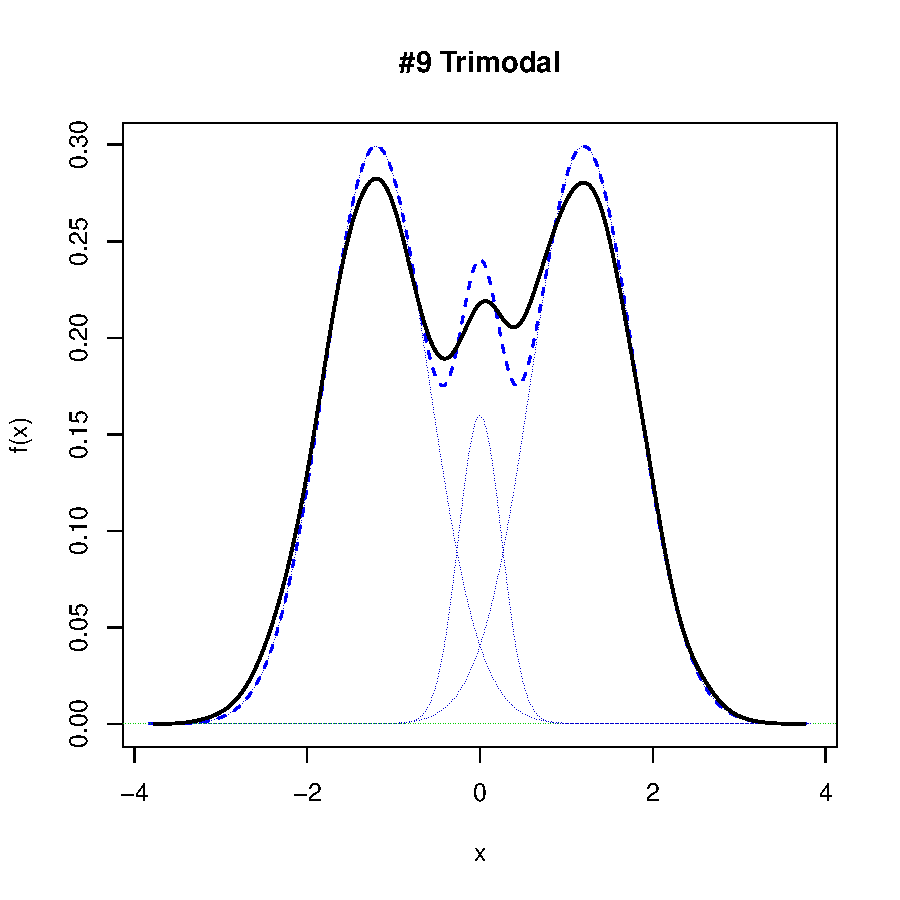
\includegraphics{chapter1-001}


then an illustration of MW examples of pathological cases


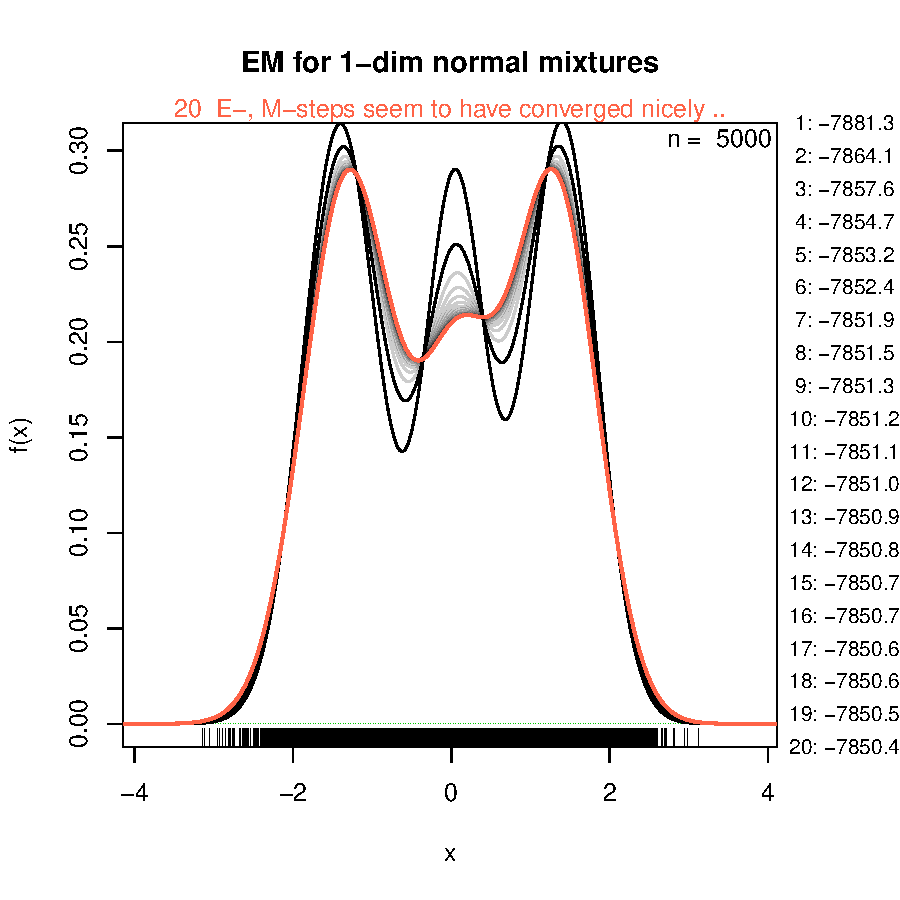
\includegraphics{chapter1-002}


yay, got figure to print. solution was use of fig=TRUE, instead of various mutations like figure=true.

here we see how change in loglik seems to stagnate. However, this does not stay that way, if we let EM run a bit further.

\begin{Schunk}
\begin{Sinput}
> r <- p.EMsteps(200, x9, nm1)
\end{Sinput}
\end{Schunk}
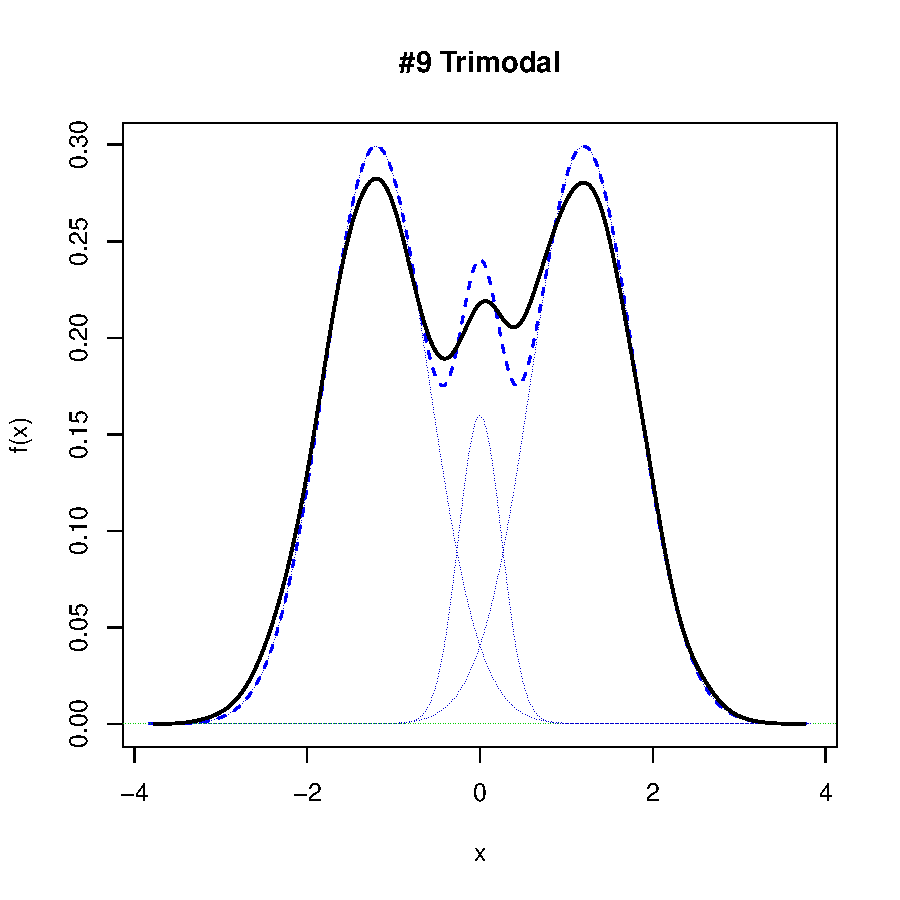
\includegraphics{chapter1-003}

to conclude example show part of mixest that shows it takes 1200 iterations to converge

In fact, it seems that the previous solution is a saddle point in the likelihood function, where EM has chronic problems continuing improvements.

should include animations?? like mix\_est\_1d.R line 249+24 lines

maybe show Marr Wand's examples of 'difficult' mixtures

give conclusion recapping the just demonstrated, and lead in for next chapter






\chapter{The {\tt norMmix} Package}

explain, that this package was written purposefully for this paper.

The norMmix package is constructed around the {\tt norMmix} object, that codifies a {\tt nor}mal {\tt M}ultivariate {\tt mix}ture model,  and the {\tt llnorMmix()} function.

quickly list contents of norMmix object

relies on {\tt optim()} generic optimizer. maximizes llnormix by varying model parameters.

since mclust is one of the more popular packages implementing the EM algo, we employ a lot of functions from mclust, to keep things around EM as similar as possible.

\section{concept of package} (this Section maybe one chapter earlier)

about Cholesky decomp as ldlt. has advantages: fast, parametrically parsimonious, can easily compute loglikelihood

maybe reread section in McLachlan about accelerating EM algo

not possible to sensibly compare normal mixtures except maybe a strange sorting algorithm using mahalanobis distance or Kullback-Leibler distance or similar(Hellinger), but not numerically sensible to integrate over potentially high-dimensional spaces.

So caomparison of algos done through throwing difficult mixtures and non-mixtures at it and hoping that norMmix finds better solutions than EM. So the criteria for "better fit" are 1. better log-likelihood 2. correct model, where EM fails.

\section{finer details of {\tt norMmix} package}




\chapter{Comparing Algotithms}

display abilities of norMmix on its own. can find correct models

maybe apply to MW[0-9] objects?

not sure


\chapter{Coclusions}

\chapter{The {\tt norMmix} Package}





\section{Introduction to the Package}

% it 1
For this thesis, an \Rp package was developed that implements the algorithm
that fits multivariate normal mixtures to given data.
\footnote{The package was written with \Rp version 3.6.1 (2019-07-05) last 
updated on 2019-10-22.}
There is a lot of unused code still in the package. These were at one point
implemented used and discarded. They are still included for demonstration.
The {\tt norMmix} package is constructed around the {\tt norMmix} object, that 
codifies a {\tt nor}mal {\tt M}ultivariate {\tt mix}ture model,  and the {\tt 
llnorMmix()} function, that calculates the log-likelihood given a model and 
data.


%% table of params
%% TODO: description of table
\begin{table}
    \centering
    \begin{tabular}{l l}
        \hline
        In Notation & In Code \\
        \hline
        $\pi_i$     & {\tt w, weights} \\
        $\Sigma$    & {\tt Sigma} \\
        $\mu$       & {\tt mu} \\
        $K$         & {\tt k} \\
        dimension   & {\tt p, dim, dims} \\
        components  & {\tt cl, components} \\
        \hline
    \end{tabular}
    \caption{Translation Table: Mathematical Notation to \Rp Code}
    \label{tab:code-notation}
\end{table}


% it 1
The package contains the following functionality:
\begin{table}
\begin{description}
    \item [norMmix] {\tt norMmix()} is the 'init-method' for 
        {\tt norMmix} objects. There exist {\tt is.norMmix} {\tt rnorMmix} and
        {\tt dnorMmix} functions.
    \item [parametrization] The main functions that handle reparametrization
        of models from and to $\pmb{LDL}^\top$ decomposition are {\tt nMm2par}
        and {\tt par2nMm}, which are inverse to each other.
    \item [MLE] The function {\tt norMmixMLE} marries the main components of 
        this package. It initializes a model and parametrizes it for use with 
        {\tt optim}
    \item [model choice] Using {\tt norMmixMLE}, the function fitnMm allows fitting 
        of multiple models and components. Functions analyzing the output of 
        this are also provided, e.g. {\tt BIC} and {\tt print} methods.
    \item [misc] There are also various methods of generics, like {\tt logLik,
        print, BIC, AIC} and {\tt nobs} as well as various {\tt print} methods.
    \item [example objects] Following the paper of \cite{Mar92} various example
        objects are provided and used for study. They follow the naming 
        convention: MW + dimension + number. for example {\tt MW213} for the 
        13-th model of dimension 2.
    \item [simulations] The purpose of this package is to study simulations. 
        there are functions provided to study large collections of evaluated 
        data. e.g {\tt epfl} %TODO: describe and give ref.
\end{description}
\end{table}

relies on {\tt optim()} generic optimizer. maximizes llnormix by varying model 
parameters.

since mclust is one of the more popular packages implementing the EM algo, we 
employ a lot of functions from mclust, to keep things around EM as similar as 
possible.

% it 1
Conceptually, at the start of a fitting algo, e.g. EM we need to initialize a
mixture object. % TODO we (will?) have translation methods to and from mclust
thereafter the paths diverge. at the heart of norMmix's functionality
lie the functions: llnorMmix and nMm2par which are in turn employed by 
norMmixMLE to funnel a mixture object into optim and give optim a function
to optimize.

also relies on {\tt mixtools} package for random generating function 
{\tt rnorMmix} using {\tt rmvnorm}.

\section{On The Development of {\tt norMmix}}

about Cholesky decomp as ldlt. has advantages: fast, parametrically 
parsimonious, can easily compute loglikelihood

%it 1

maybe reread section in McLachlan about accelerating EM algo

not possible to sensibly compare normal mixtures except maybe a strange sorting 
algorithm using Mahalanobis distance or Kullback-Leibler distance or similar
(Hellinger), but not numerically sensible to integrate over potentially 
high-dimensional spaces.

%% TODO: explain comparison


general list of (not necessarily mathematical) dead-ends in the development 
life of the norMmix package.
argue why this is in this section?? because, as a BScT, the learning is as much
part of the research as the results.


% it 1
One dead-end was the parametrization of the weights of a mixture using the 
{\tt logit} function.

\begin{Schunk}
\begin{Sinput}
> logit <- function(e) {
+     stopifnot(is.numeric(e) ,all(e >= 0), all.equal(sum(e),1))
+     qlogis(e[-1L])
+ }
> logitinv <- function(e) {
+     if (length(e)==0) {return(c(1))}
+     stopifnot(is.numeric(e))
+     e<- plogis(e)
+     sp. <- sum(e)
+     w <- c((1-sp.), e)
+ }
\end{Sinput}
\end{Schunk}

This uses the logistical function {\tt logis} to transform to reduce the number
of weights from $K$ to $K-1$. Much like {\tt clr1}, given a list of weights 
{\tt logit} will transform them and {\tt logitinv} will correctly reverse the 
transformation. However, unlike {\tt clr1}, it will not transform an arbitrary 
list of length $K-1$ into a valid weight parameter. For example:

\begin{Schunk}
\begin{Sinput}
> w <- runif(7); ret <- logitinv(w)
> ret
\end{Sinput}
\begin{Soutput}
[1] -3.2617309  0.6306458  0.5682759  0.5602498  0.6616009  0.6906020  0.5707690
[8]  0.5795875
\end{Soutput}
\end{Schunk}

The issue here is that the last line of {\tt logitinv}, which is necessary to 
sum to one, but results in a negative value in {\tt ret[1]} which is not a 
valid weight. The underlying issue is that not every tuple in $\R^{K-1}$ is 
a result of {\tt logit}.

The option to use {\tt logit} is still an argument to {\tt norMmixMLE} by 
specifying {\tt trafo="logit"}, but it shouldn't be used.


% it 1
Another issue during development cropped up during fitting of high dimensional
data. We studied the dataset {\tt SMI.12} from the package {\tt copula}:

\begin{Schunk}
\begin{Sinput}
> data(SMI.12, package="copula")
> str(SMI.12)
\end{Sinput}
\begin{Soutput}
 num [1:141, 1:20] 16.1 15.7 15.7 16.1 16.6 ...
 - attr(*, "dimnames")=List of 2
  ..$ : chr [1:141] "2011-09-09" "2011-09-12" "2011-09-13" "2011-09-14" ...
  ..$ : chr [1:20] "ABBN" "ATLN" "ADEN" "CSGN" ...
\end{Soutput}
\end{Schunk}

A consequence of high dimensions is that matrix multiplication is no longer
very stable. As a result, the covariance matrices produced by our own 
implementation of the EM-algorithms m-step ({\tt mstep.nMm}) were not positive
definite.
In the case of {\tt SMI.12}, several covariance matrices are degenerate, which
results in cancellation error with near-zero entries.
We attempted to correct this with the function {\tt forcePositive}, which 
simply tries to set $\pmb{D}$ in $\pmb{LDL}^\top$ greater than zero.
This didn't resolve the issue, since a non-negligible part of the numerical
error was in the $\pmb{L}$ matrix and the resultant covariance matrix was still
not positive definite.

We eventually resolved this issue by abandoning our own implementation and 
using the functions from the {\tt Mclust} package. Not only were these 
numerically stable they were also able to differentiate between models, whereas
ours would assume VVV for every fit.

testing of mvtnorm as proof that ldlt is in fact faster parametrization

mention, that there may be faster ways to apply backsolve. 
quote knuth about premature optimization?

\section{Demonstration}

Mention, that mclust doesn't depend on seed(double check) and therefore norMmix has 
'advantage' of 'confidence intervals'. We can run 50 simulations and see if there
might be more sensible clusters.


% it 1
demonstrate things; essentially put .Rd example sections here

\chapter{Comparing Algorithms}


% it 1
With the {\tt norMmix} package explained, we can turn to comparing it to 
existing methods. As previously stated, the implementation representing the 
EM-algorithm is the {\tt mclust} package. It will be used with very little 
deviation from out-of-the-box, safe for restriction of the covariance models.
This is done, so we can compare like with like.
The specific command that performs the EM-algorithm is:

\begin{Schunk}
\begin{Sinput}
>     mclust::Mclust(x, G=cl, modelNames=mo)$BIC
\end{Sinput}
\end{Schunk}

Where {\tt cl} is a vector of integers of however many components we are trying 
to fit and {\tt mo} are the model names:

\begin{Schunk}
\begin{Soutput}
 [1] "EII" "VII" "EEI" "VEI" "EVI" "VVI" "EEE" "VEE" "EVV" "VVV"
\end{Soutput}
\end{Schunk}

The {\tt \$BIC} element of the results is taken as the main tool for model 
selection, as it is advertised in the package authors paper \cite{Scr16}.

There is however a small but crucial change applied to these results.
The {\tt mclust} package authors have flipped the definition of the BIC to mean:
\begin{equation} 
    2 ln(\hat{L}) - ln(n) \#\{par\}
\end{equation}
instead of the more common
\begin{equation} 
    ln(n) \#\{par\} - 2 ln(\hat{L})
\end{equation}
Where $n$ is the number of observations, \#\{par\} is the cardinality of the 
parameter vector and $\hat{L}$ is the estimated log-likelihood.

So, even if not explicitly mentioned, we use the negative of the values returned
by {\tt mclust}.

Another thing that should be stated before all else is the difference in 
initialization between {mclust}'s pre-clustering and CLARA. CLARA is dependent
on random number generators (RNG). As such, unless a fixed seed is chosen, 
every iteration of CLARA will return a different result. Unlike {\tt mclust}, 
which will, for given data, always return the same results. The effect on the 
following findings is that results will spread out for data obtained from 
CLARA results.


% it 1
First, we illustrate the structure of the graphical results we will be 
presenting hereafter. The basic shape of the plots will be the BIC value 
plotted against the number of components. This is in line with {\tt mclust}'s
manner of visualizing data, however since our method is to some extent RNG 
dependent, we are forced to display multiple runs of the algorithm on the same
graph. Therefore we split the plot according to covariance model, putting 10
models in 10 graphs in a plot. Here an example:


\begin{figure}[h!]
    \begin{Rgraph}[0.9]
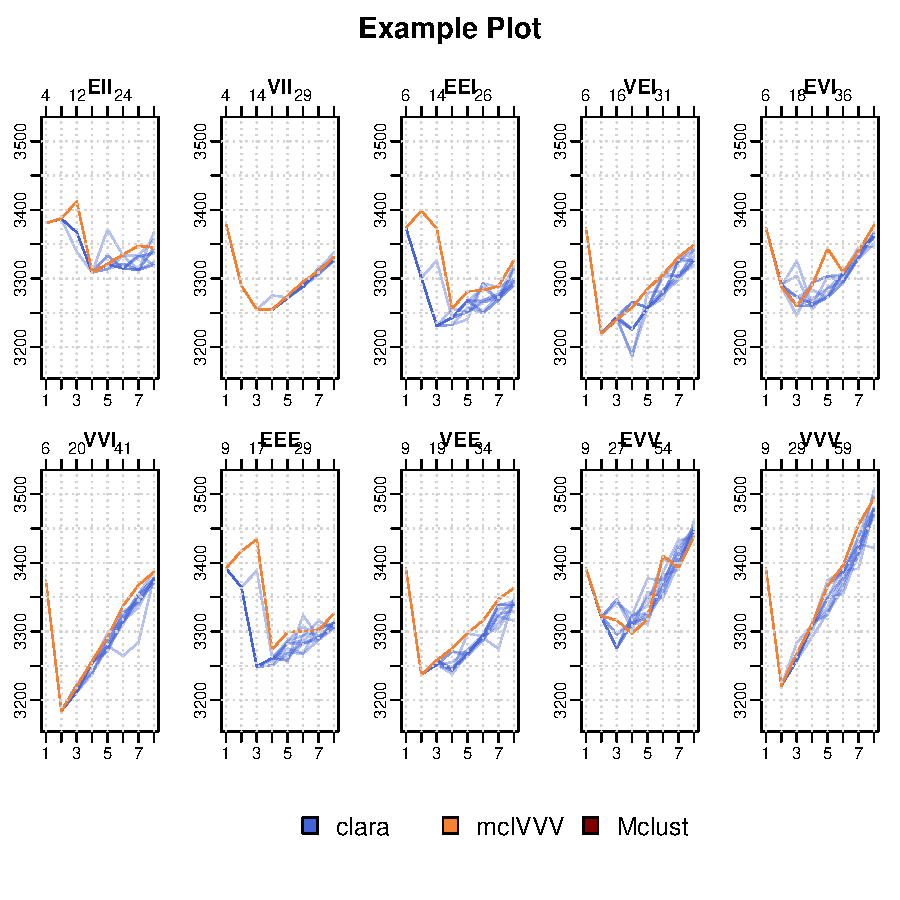
\includegraphics{chapter3-bicplotdemoplot}
    \caption{Example of Comparison Plot}
    \label{fig:ExPlot}
    \end{Rgraph}
\end{figure}

As can be seen from the formula of the BIC value, lower is better. When 
selecting a model based on BIC, we take the model and component with the 
lowest value to be the best fitting model. Although this may not necessarily
the 'correct' model, that is, the model from which the data arises.

There are many ways in which this type of model selection might miss the 
correct model, for example by 'gluing together' multiple components into one,
or covering the dataset in a 'patchwork' of smaller components, to name a few.

We will discuss them as they arise in the following analysis of simulations

The simulations were set up very simply. An \Rp script was written and in each
the {\tt norMmix} package is loaded, the datasets are defined and {\tt fitnMm}
was applied a number of times. An example script can be found in the appendix
\ref{App:sims}.

A few things of interest are what happens:
\begin{itemize}
    \item To time needed for the simulation
    \item When we vary the sample size of the data sets.
    \item When the generating mixture is 'difficult'.
    \item When the data does not arise from a normal mixture.
\end{itemize}

The data used here should have been provided along with this thesis in digital 
form in a folder called {\tt /simulations}


\section{Time Analysis}


The data used here is taken from the subfolder {\tt /simulations/2time}.
From these, the system time was extracted and analyzed as can be gleaned from
the following code. In it, we apply \Rp's {\tt lm} function for fitting linear 
models to the times returned by the function call:
\begin{Schunk}
\begin{Sinput}
>     system.time(norMmixMLE(x, ...))[[1]]
\end{Sinput}
\end{Schunk}
We make here a choice that does not preserve any generality, as 
{\tt system.time} produces more results, that could hold important information.
However, since there is quite some measurement error to be expected as time 
approaches zero, we will content ourselves with lower expectations to the 
accuracy of the following results.


\begin{Schunk}
\begin{Sinput}
>     library(norMmix, lib.loc="~/ethz/BA/norMmix.Rcheck/")
>     # change this dir to whereever the simulations are saved
>     mainsav <- normalizePath("~/ethz/BA/Rscripts/")
>     savdir <- file.path(mainsav, "2time")
>     filelist <- list.files(savdir, pattern=".rds")
>     filelist <- grep("mcl.rds", filelist, invert=TRUE, value=TRUE)
>     f <- lapply(file.path(savdir,filelist), function(j) readRDS(j)$fit)
>     times <- unlist(lapply(f, function(j) extracttimes(j)[,,1]))
>     dims <- unlist(lapply(f, function(j) attr(extracttimes(j), "p")))
>     size <- unlist(lapply(f, function(j) attr(extracttimes(j), "n")))
>     ddims <- rep(dims, each=80)
>     ssize <- rep(size, each=80)
>     pars <- unlist(lapply(f, npar))
>     r <- lm(times ~ pars + ddims + ssize)
>     summary(r)
\end{Sinput}
\begin{Soutput}
Call:
lm(formula = times ~ pars + ddims + ssize)

Residuals:
   Min     1Q Median     3Q    Max 
-86.89  -7.45  -1.55   6.30 556.32 

Coefficients:
              Estimate Std. Error t value Pr(>|t|)    
(Intercept) -1.727e+01  8.274e-01  -20.87   <2e-16 ***
pars         9.729e-01  1.056e-02   92.16   <2e-16 ***
ddims       -3.749e+00  2.216e-01  -16.92   <2e-16 ***
ssize        9.258e-03  3.887e-04   23.82   <2e-16 ***
---
Signif. codes:  0 ‘***’ 0.001 ‘**’ 0.01 ‘*’ 0.05 ‘.’ 0.1 ‘ ’ 1

Residual standard error: 21.57 on 7916 degrees of freedom
Multiple R-squared:  0.559,	Adjusted R-squared:  0.5588 
F-statistic:  3344 on 3 and 7916 DF,  p-value: < 2.2e-16
\end{Soutput}
\end{Schunk}

The necessary time appears to be well explained by the parameter count.
The purpose of this thesis is not to conduct complexity analysis, so we will
leave it at this, satisfying our curiosity with a cursory look in figure 
\ref{fig:time}, where we plot system time against parameter length.

\begin{figure}[h!]
    \begin{Rgraph}[0.9]
\begin{Schunk}
\begin{Sinput}
>     plot(times~pars, log="xy", yaxt="n", xaxt="n", type="n")
>     legend("bottomright", legend=c("MW214", "MW34","MW51"),
+            fill=nMmcols[c(3,4,2)])
>     points(times[1:(80*30)]~pars[1:(80*30)], 
+            log="xy", yaxt="n", xaxt="n", col=nMmcols[3])
>     points(times[(80*30+1):(80*60)]~pars[(80*30+1):(80*60)]
+            , log="xy", yaxt="n", xaxt="n", col=nMmcols[4])
>     points(times[(60*80+1):(80*90)]~pars[(60*80+1):(80*90)], 
+            log="xy", yaxt="n", xaxt="n", col=nMmcols[2])
>     grid()
>     sfsmisc::eaxis(1)
>     sfsmisc::eaxis(2)
\end{Sinput}
\end{Schunk}
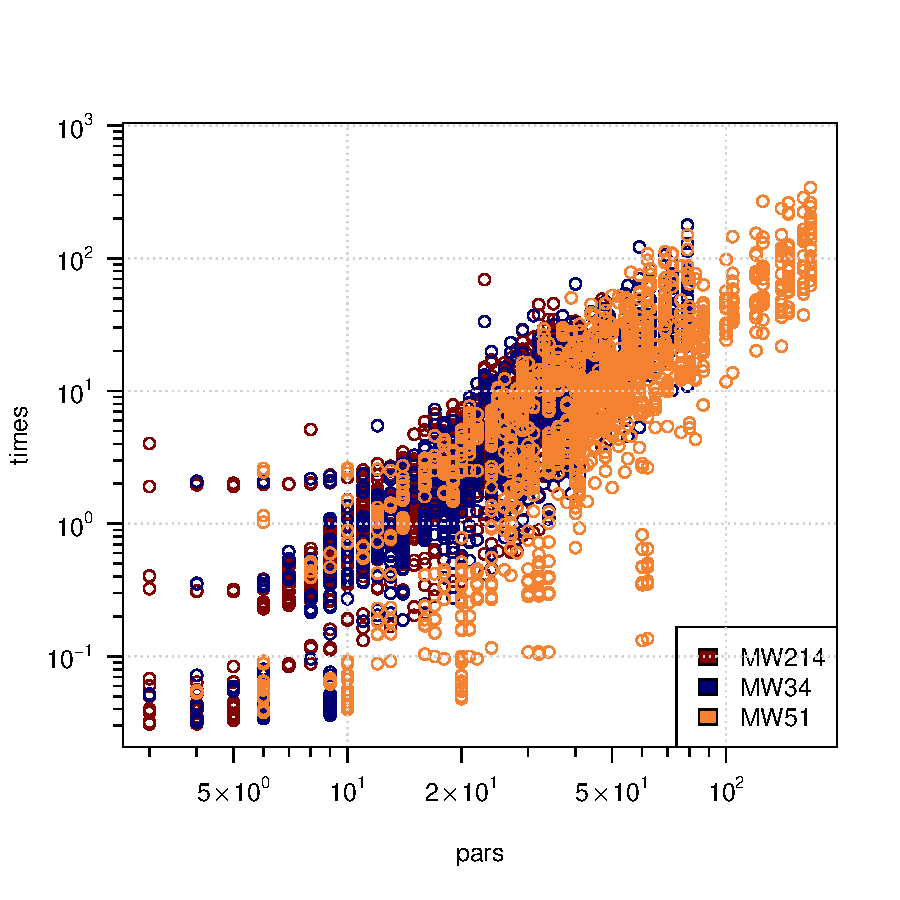
\includegraphics{chapter3-figtime}
    \caption{Log-log Plot of System Time against Parameter Length}
    \label{fig:time}
    \end{Rgraph}
\end{figure}

We can see that time is almost one to one proportional to parameter length.
It should be noted, that {\tt MW51} is a very simple mixture. It is therefore 
sensible, that MLE should find an optimum faster.

\clearpage

\section{Behaviour in {\tt n}}
\label{sec:ben}

% it 1
What we would expect and like to see as we increase sample size, is a decrease
in scattering of BIC values. To that end we again use simulation data 
{\tt /2time}. In particular we show here the results of fitting to mixture 
model {\tt MW34}, shown in figure \ref{fig:MW34}. The graphs 
\ref{fig:bicmw34first} and \ref{fig:bicmw34second} show three columns
of BIC plots, each representing different sample sizes, with 
$n = \{500, 1000, 2000\}$ respectively. Furthermore, the BIC values were 
divided by the samplesize, to normalize the values to an equal scale.

\begin{figure}[h]
    \begin{Rgraph}[0.9]
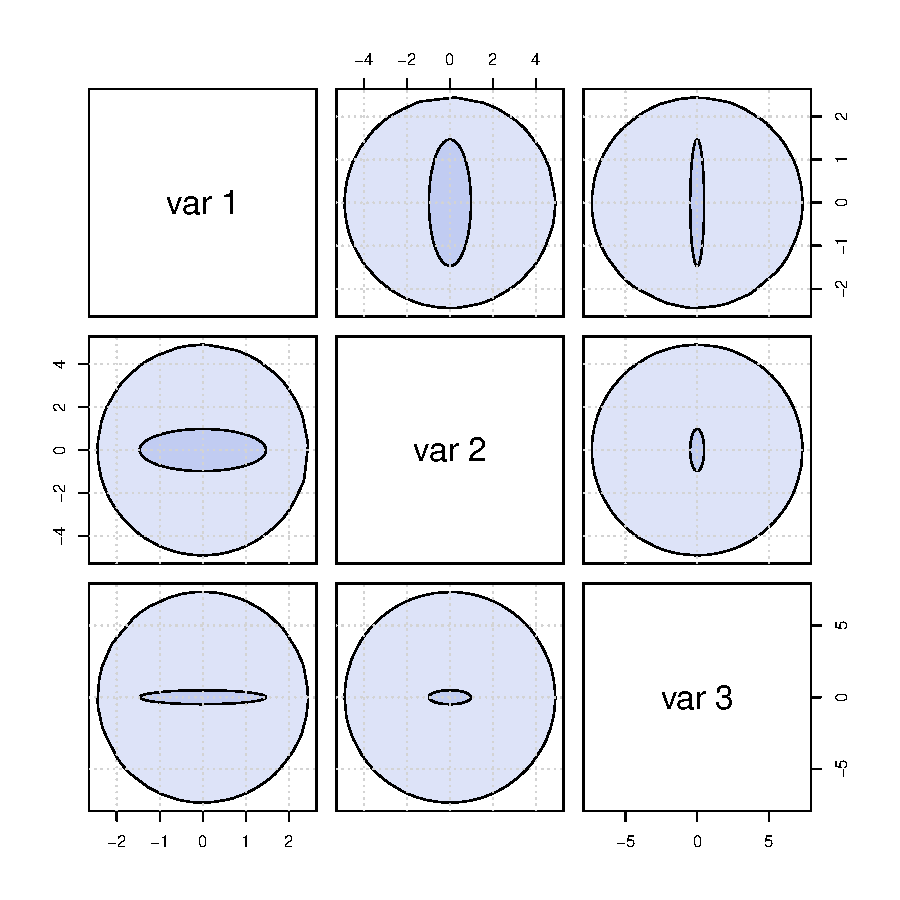
\includegraphics{chapter3-figMW34}
    \caption{The mixture model {\tt MW34}, a three dimensional, two component
             mixture with one smaller, lesser weighted component inside a 
             smaller one.}
    \label{fig:MW34}
    \end{Rgraph}
\end{figure}


\begin{figure}[h!]
    \begin{Rgraph}[0.9]
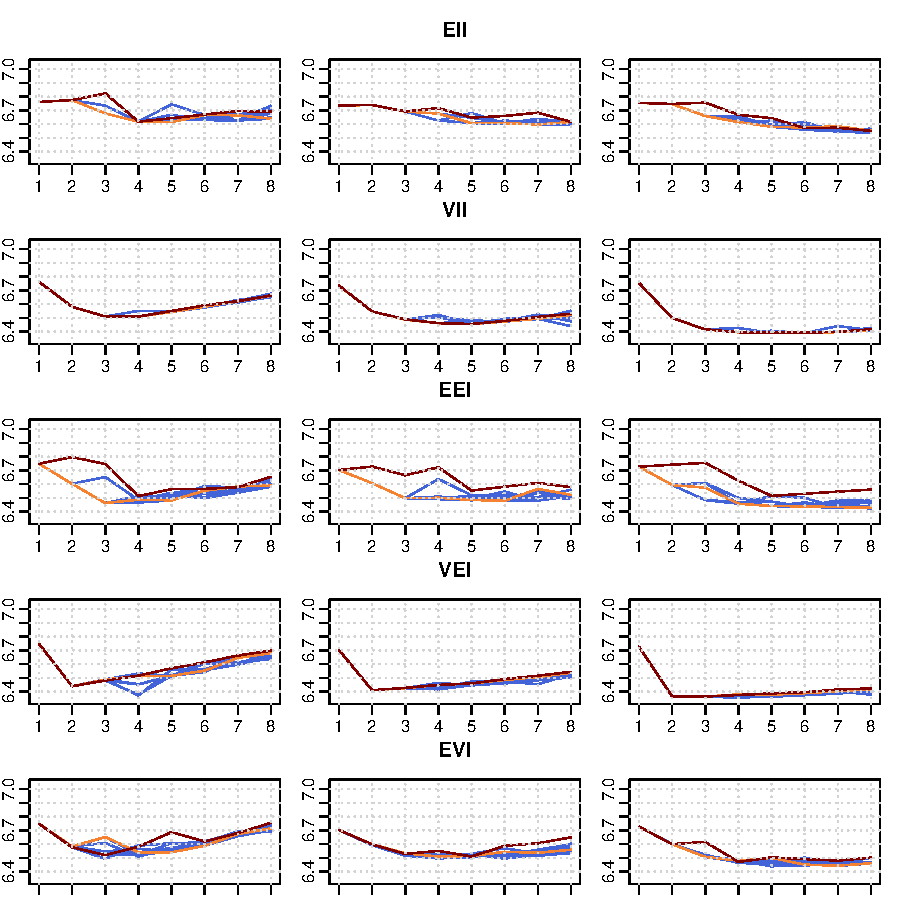
\includegraphics{chapter3-figmw34bicfirst}
    \caption{BIC values of {\tt MW34} with $n=2000$}
    \label{fig:bicmw34first}
    \end{Rgraph}
\end{figure}

As can be seen the desired effect is achieved. Of note are the behaviour of 
the model {\tt VEI}, where the increase in observation corrects a selection
error appearing at $n=500$. Furthermore, the correct model {\tt VVI} exhibits
a very tight grouping. The instances where {\tt mclust} is better than 
{\tt norMmix} are quite infrequent.

This type of analysis was also conducted with mixture objects {\tt MW214} and 
{\tt MW51}, but were ommited due to the lack of clear results. They are 
provided in the appendix \ref{app:ben}, with brief discussions.

\begin{figure}[h!]
    \begin{Rgraph}[0.9]
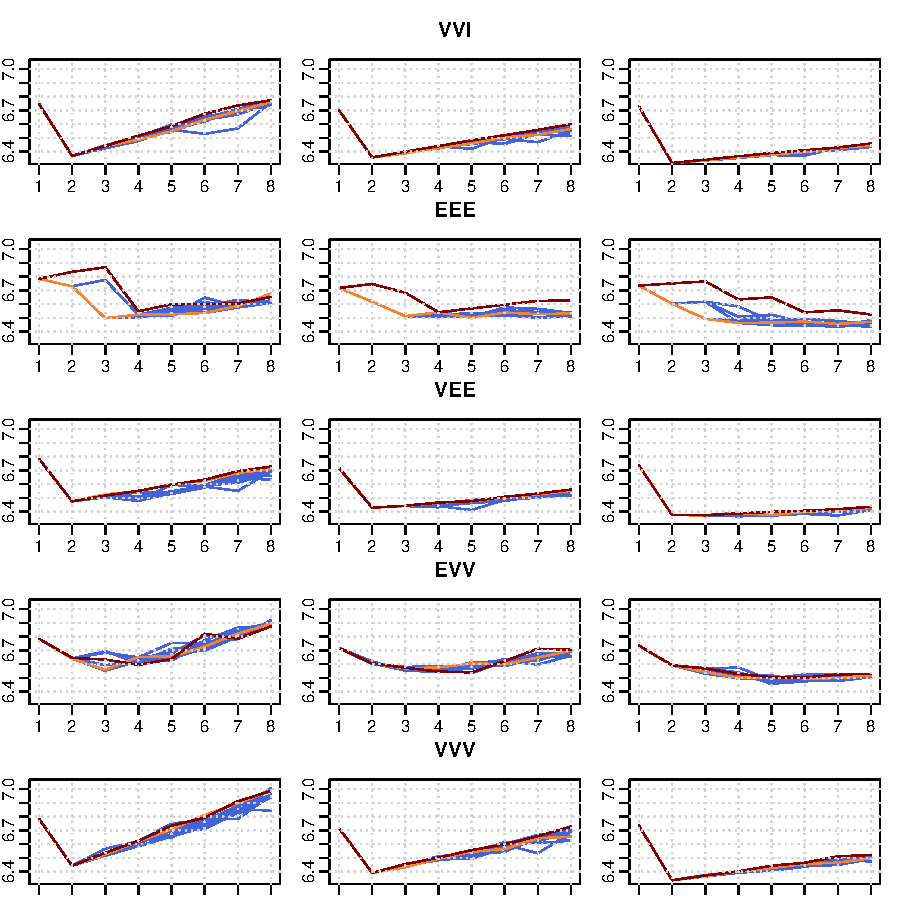
\includegraphics{chapter3-figmw34bicsecond}
    \caption{BIC values of {\tt MW34} with $n=2000$}
    \label{fig:bicmw34second}
    \end{Rgraph}
\end{figure}

\clearpage

\section{Difficult Mixtures}
\label{sec:dif}

% it 1
In this section we analyze the two mixtures given by {\tt MW215} and {\tt MW214}.
These are a trimodal and a claw-like distribution. These types of mixtures were 
also discussed in \cite{Mar92}, in the univariate case, where they proved to be 
difficult to fit.

First the trimodal mixture shown in figure \ref{fig:MW215}. The difficulty 
lies in the components of various sizes lying close together.

\begin{figure}
\begin{Rgraph}[0.9]
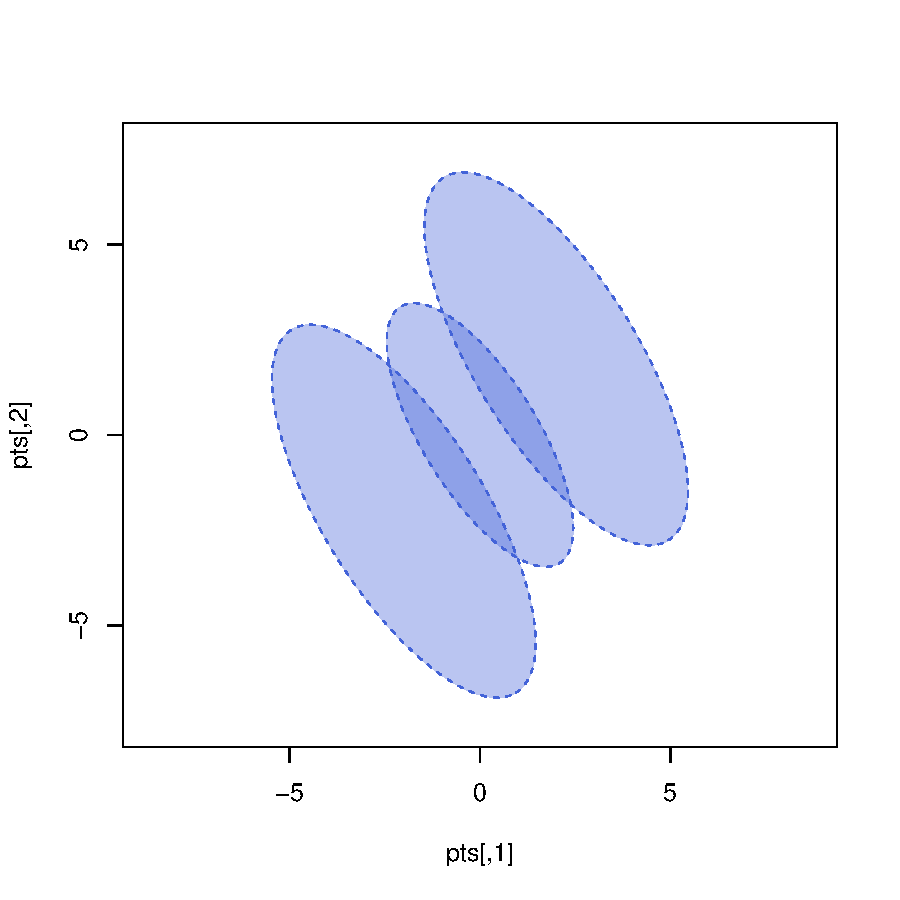
\includegraphics{chapter3-figMW215}
    \caption{Trimodal mixture {\tt MW215}. Three equally weighted, oriented, and
             shaped components of different volumes along the diagonal}
    \label{fig:MW215}
\end{Rgraph}
\end{figure}


\begin{figure}[h!]
    \begin{Rgraph}[0.9]
\begin{Schunk}
\begin{Sinput}
>     compplot(clarabic, mclbic, mclustbic, main="Fit of MW34")
\end{Sinput}
\end{Schunk}
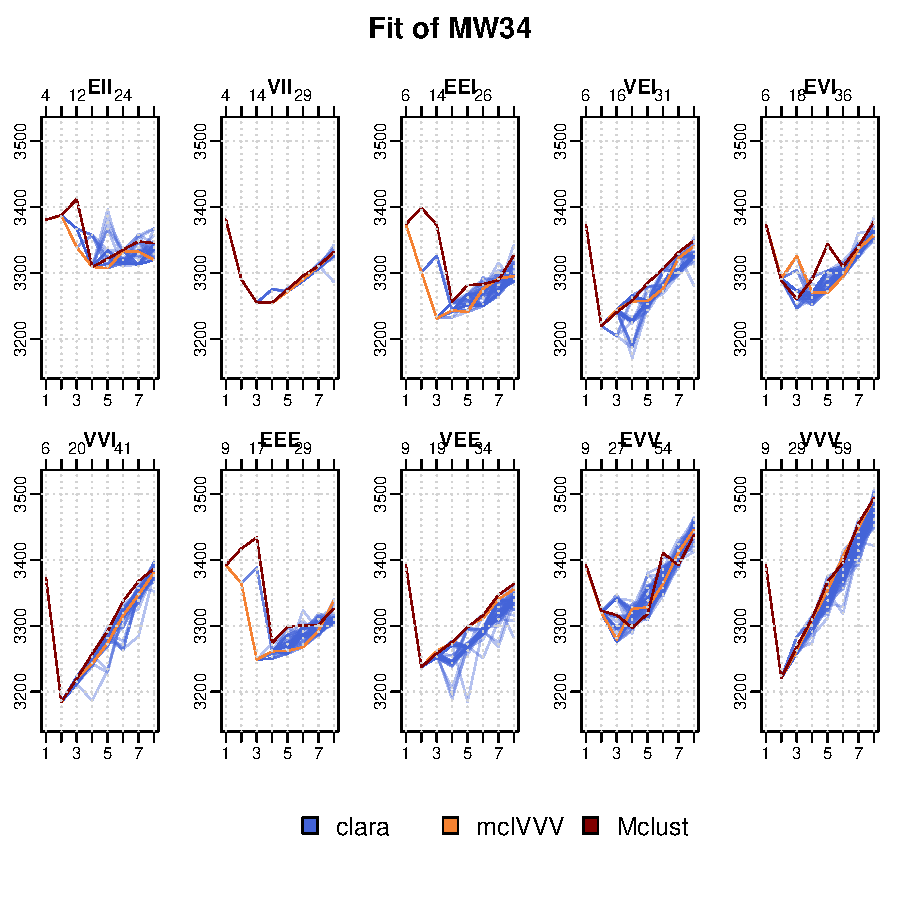
\includegraphics{chapter3-figMW34bic}
    \caption{BIC values of {\tt MW34}, correct: {\tt model="VVI", k=2}}
    \label{fig:bicMW34}
    \end{Rgraph}
\end{figure}

We can see, that in many cases both initialization methods {\tt clara} and
{\tt mclVVV} manage to achieve a lower BIC value than {\tt mclust}. Although in
the case of the correct model and cluster, {\tt k=3, model="VEE"} the three 
algorithms coincide.

A search for best values reveals, that the best models selected are in almost 
all cases the correct model.

\begin{Schunk}
\begin{Soutput}
     model   count
[1,] "2 VVI" "49" 
[2,] "4 VEI" "1"  
\end{Soutput}
\end{Schunk}

The one incorrect model looks like this:

\begin{figure}[h]
    \centering
    \begin{minipage}{0.45\textwidth}
        \centering
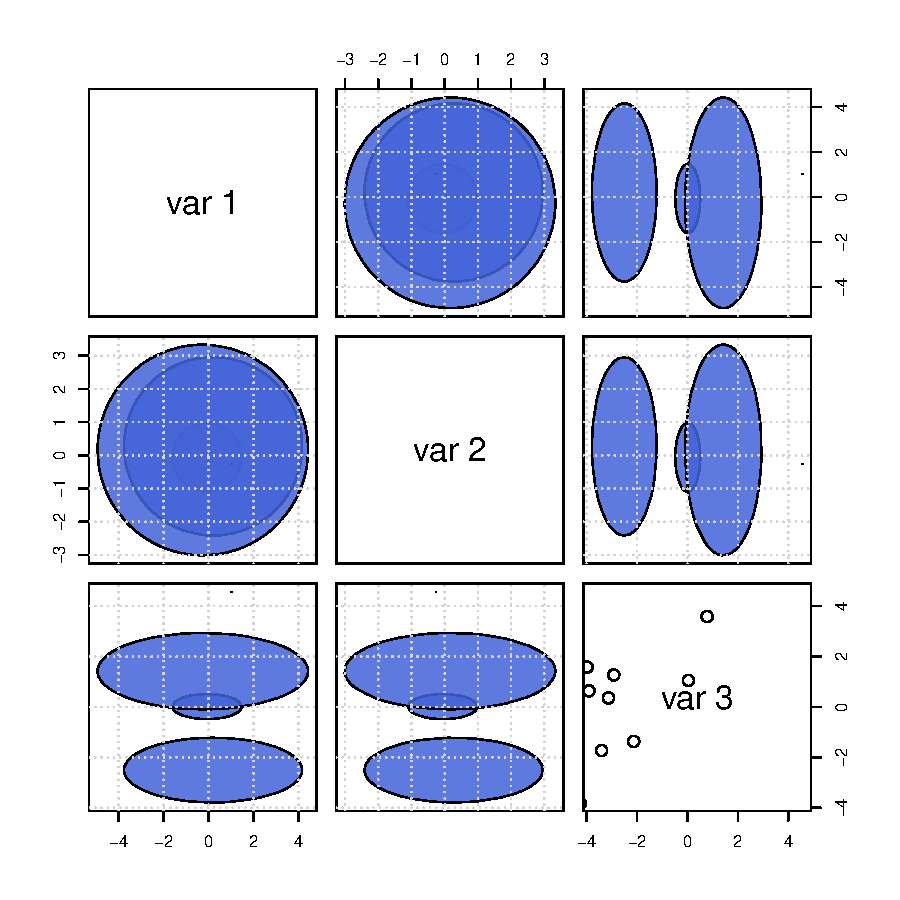
\includegraphics{chapter3-figerrorMW215}
    \end{minipage}
    \begin{minipage}{0.45\textwidth}
        \centering
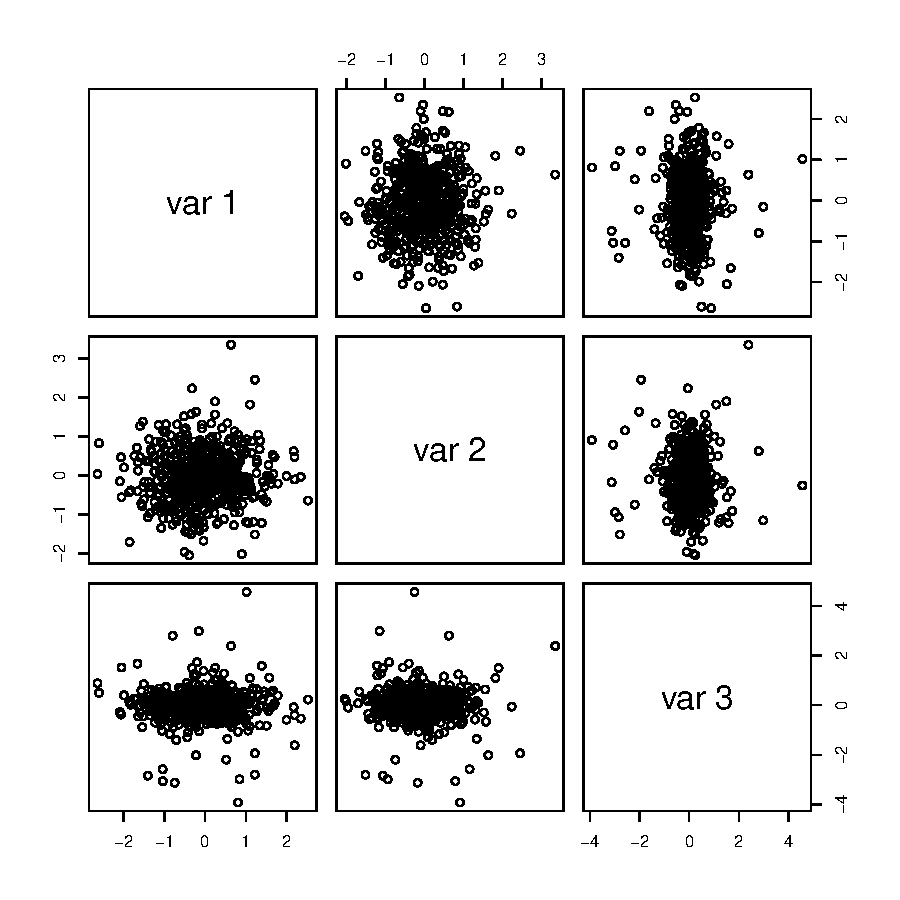
\includegraphics{chapter3-figerrorMW215x}
    \end{minipage}
\end{figure}

and has the weights: 0.942, 0.0321, 0.0244, 0.002. This is an issue of 
spurious clusters. These are clusters formed by a low number of datapoints
conjoined into a component with small determinant of its covariance matrix.
It is a flaw in the {\tt norMmix} package, that is not adressed.

Now for the claw-like mixture, {\tt MW214}. It is a mixture of six components
and a very simple {\tt "VII"} covariance model. A large encompassing component
and five smaller, lightly wheighted components closely together along the 
diagonal. The inherent difficulty lies in the fact that the components overlap
and are close together as well. It is shown in figure \ref{fig:MW214}.

\begin{figure}[h!]
    \begin{Rgraph}[0.9]
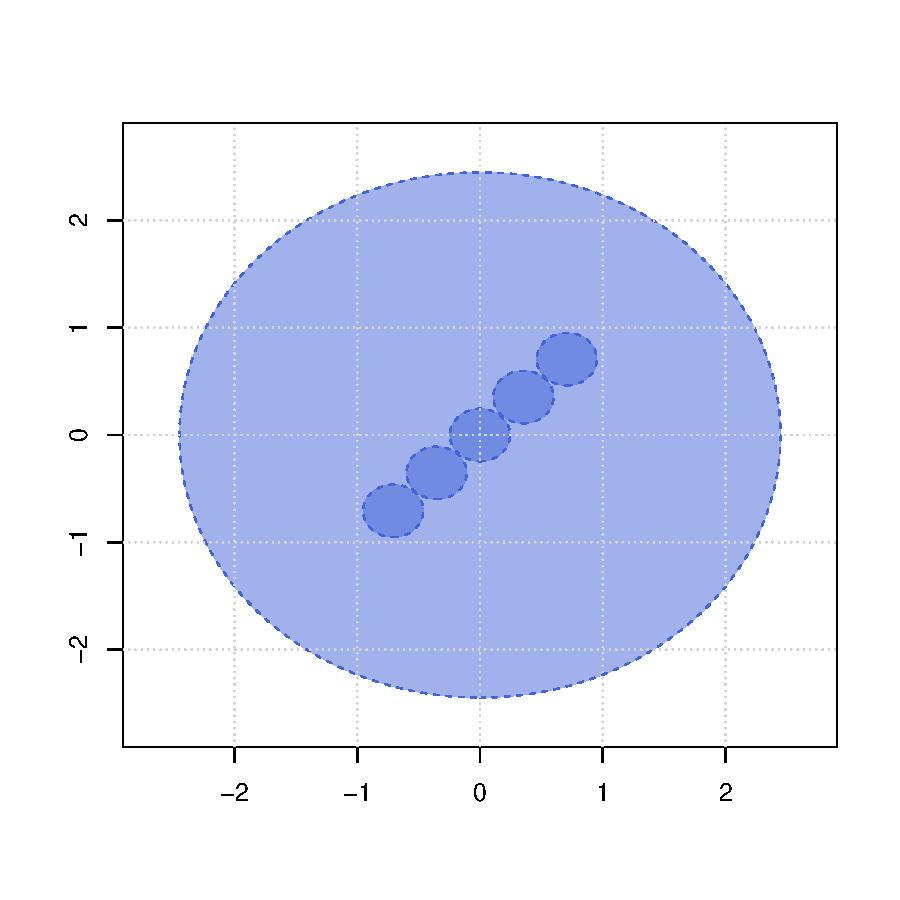
\includegraphics{chapter3-figMW214}
    \caption{Claw-like mixture}
    \label{fig:MW214}
    \end{Rgraph}
\end{figure}



\begin{figure}[h!]
    \begin{Rgraph}[0.9]
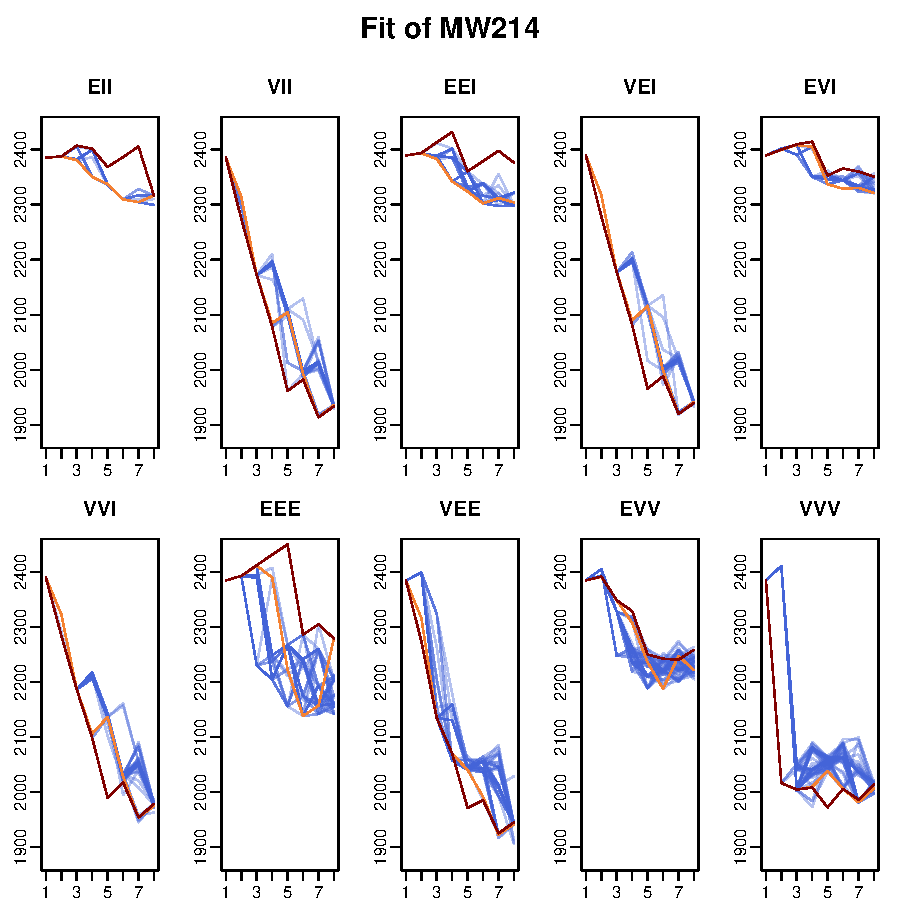
\includegraphics{chapter3-figMW214bic}
    \caption{BIC values of claw-like mixture. Best fit: {\tt model="VEE", k=8},
             correct: {model="VII", k=6}}
    \label{}
    \end{Rgraph}
\end{figure}

We take a look at the best results per simulation again:

\begin{Schunk}
\begin{Soutput}
     model   count
[1,] "8 VII" "27" 
[2,] "7 VEE" "8"  
[3,] "7 VEI" "8"  
[4,] "7 VII" "4"  
[5,] "8 VEE" "3"  
\end{Soutput}
\end{Schunk}

And here are the ten best values:

\begin{Schunk}
\begin{Soutput}
      comp model BIC               
 [1,] "8"  "VEE" "1905.61014581771"
 [2,] "8"  "VEE" "1907.24944742008"
 [3,] "8"  "VEE" "1913.57109788463"
 [4,] "7"  "VII" "1913.68061849043"
 [5,] "7"  "VII" "1913.68062199219"
 [6,] "7"  "VEE" "1916.40190209225"
 [7,] "7"  "VEE" "1916.40195605402"
 [8,] "7"  "VEI" "1918.15484419568"
 [9,] "7"  "VII" "1918.35924550811"
[10,] "7"  "VII" "1918.4864952664" 
\end{Soutput}
\end{Schunk}


Here some examples of fitted mixtures:

\begin{figure}[h!]
    \begin{Rgraph}[0.9]
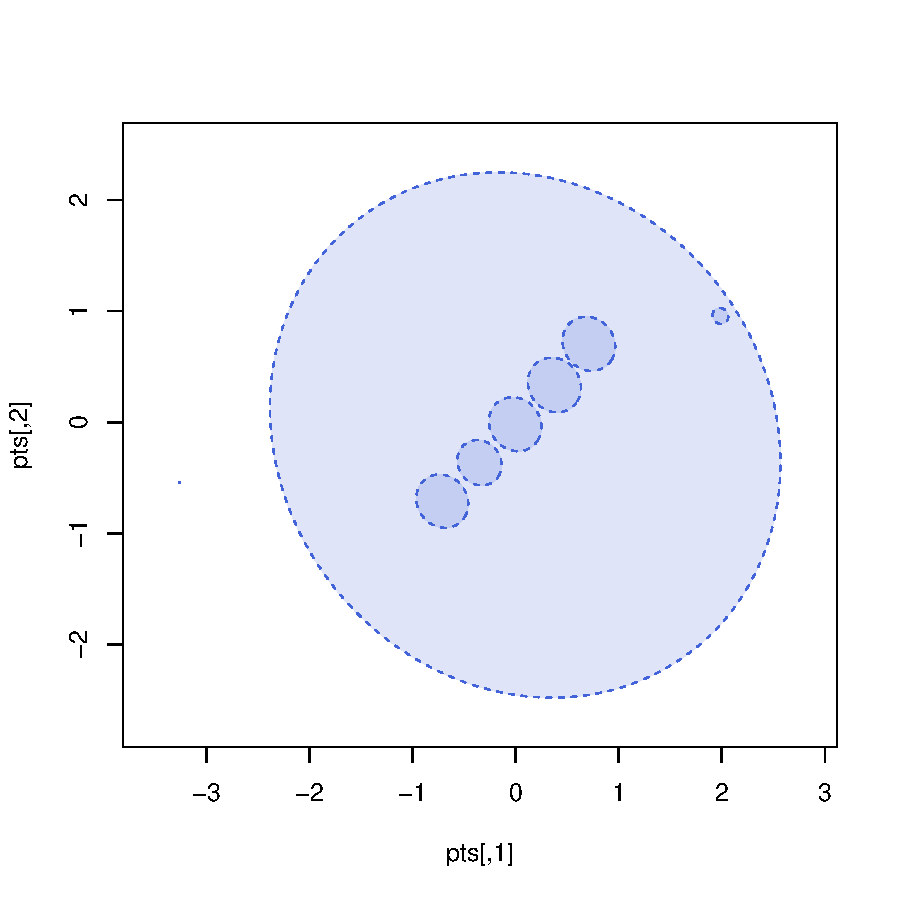
\includegraphics{chapter3-fig214fit}
    \caption{Best Fit over $n=$ model selections. {\tt model="VEE", k=8} Correct
             model {\tt model="VII", k=6}. Of Note Here are the Spurious 
             Clusters Appearing.}%whats n?? should be verbose
    \label{fig:MW214bestfit}
    \end{Rgraph}
\end{figure}

\begin{figure}[h]
    \begin{Rgraph}[0.9]
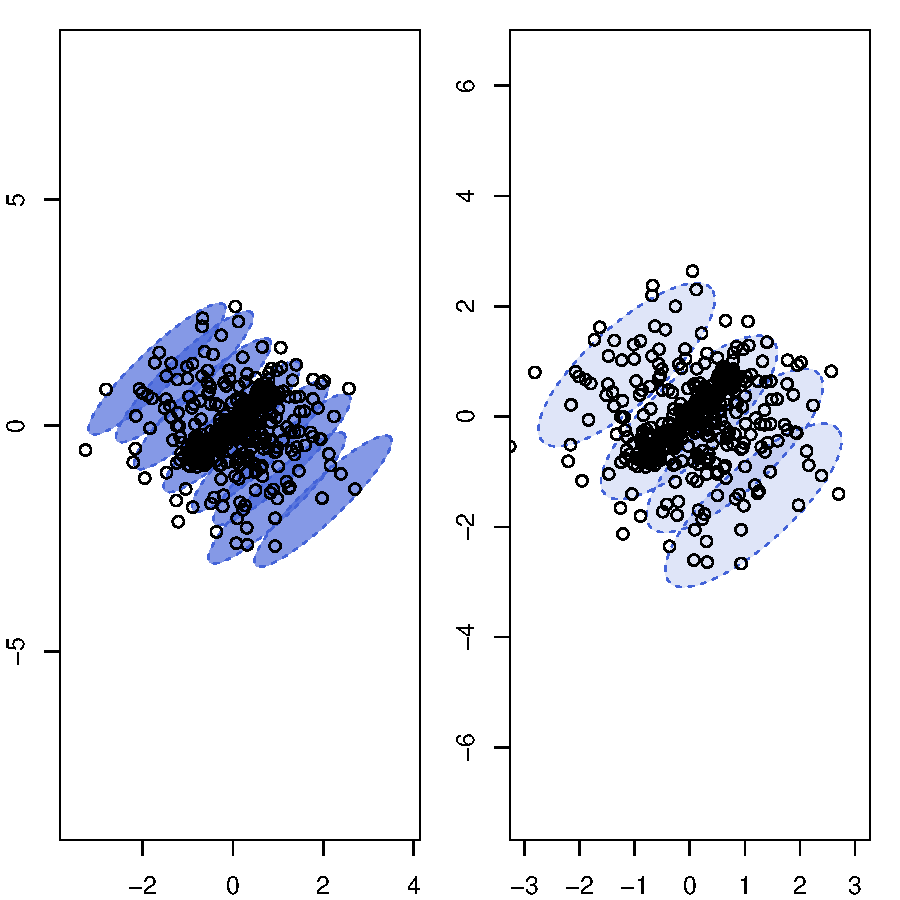
\includegraphics{chapter3-fig214fit2}
    \end{Rgraph}
    \caption{Two of the better clusters. They both follow the 'patchwork'
             covering strategy, laying patches of components over the dataset}
    \label{fig:214fit2}
\end{figure}

We can see, that, subtracting the obvious hiccups of the small erroneous
components, {\tt norMmix} has correctly found the 'intended' 
distribution. This is remarkable, given the small sample size and difficulty of 
distribution. As can be seen in figure \ref{fig:214fit2}, there are mistakes in
the near best clusters, where the data is overlayed with a 'patchwork' of 
components.

\clearpage

\section{Nonnormal Mixtures}

here 2smi and 2var, maybe others as well.
here mention that coverage of algo is extremely patchy.
here 2smi:
Using only datasets generated from the intended model can hide important 
structural errors in an algorithm. To that end we also applied {\tt norMmix}
to nonnormal data to see if any erratic behaviour appears.

The data used are the {\tt SMI.12} and {\tt loss} from the package {\tt copula}
\cite{cop18}, as well as the {\tt iris} data included in base \Rp.

We begin with the {\tt SMI.12} dataset, that has already been discussed 
previously. This also doubles as high-dimensional analysis, as it is 20 
dimensional.


\begin{figure}[h!]
    \begin{Rgraph}[0.9]
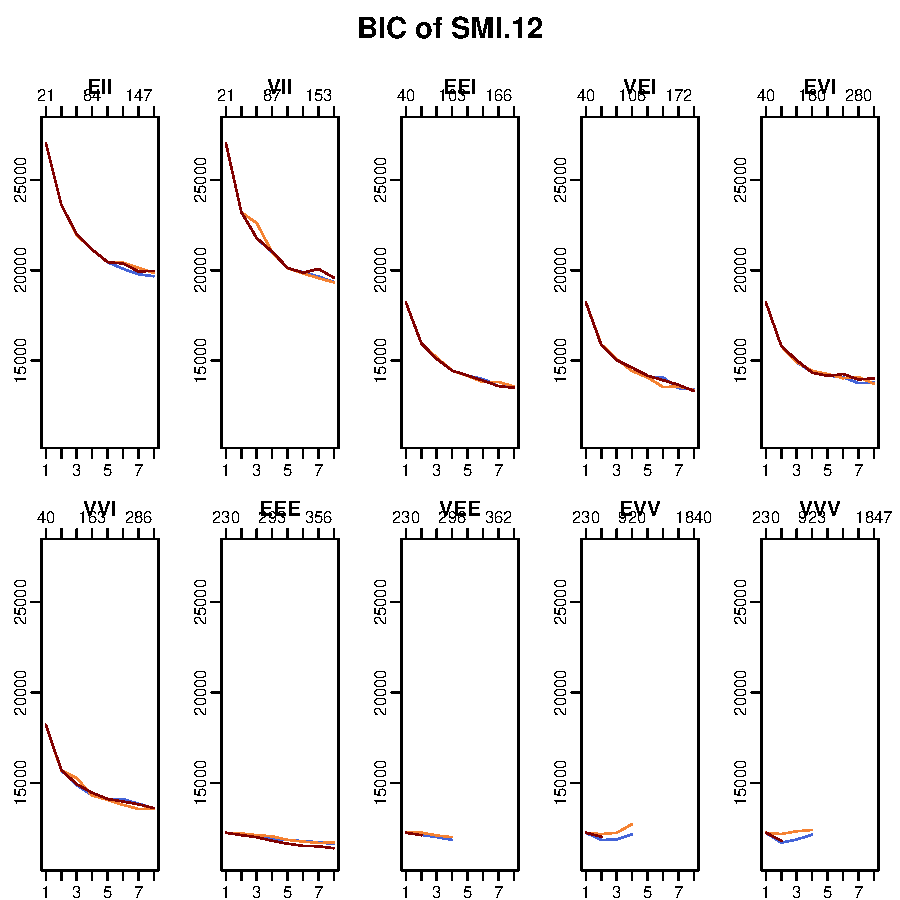
\includegraphics{chapter3-2smiplot}
    \end{Rgraph}
    \caption{The BIC values of the {\tt SMI.12} data. The blue line representing
             the {\tt clara} values is covered by the other lines. The last 
             three models are not plotted for all component sizes, as the 
             algorithm returns an error if the fitting problem is ill defined.}
    \label{}
\end{figure}

While not very spectacular, the graphs show that even at large parameter
counts our algorithm closes in on the same values as {\tt mclust}.
At these dimensions it is difficult to compare if these are actually 
equal, or even similar fits, but going by BIC values, it is at the very 
least equally viable as a working model.
The last three models are not fully plotted for all components. The reason for 
this is that {\tt norMmix} relies on {\tt mclust} in its m-step. The 
{\tt mclust} package halts computation when the clustering problem is badly 
posed. In this instance the problem is that the parameter count is much larger 
than the number of observations.

To illustrate, here are the parameter sizes for this simulation:

\begin{Schunk}
\begin{Soutput}
  EII VII EEI VEI EVI VVI EEE VEE  EVV  VVV
1  21  21  40  40  40  40 230 230  230  230
2  42  43  61  62  80  81 251 252  460  461
3  63  65  82  84 120 122 272 274  690  692
4  84  87 103 106 160 163 293 296  920  923
5 105 109 124 128 200 204 314 318 1150 1154
6 126 131 145 150 240 245 335 340 1380 1385
7 147 153 166 172 280 286 356 362 1610 1616
8 168 175 187 194 320 327 377 384 1840 1847
\end{Soutput}
\end{Schunk}

{\tt SMI.12} has 141 observations, which is exceeded by the parameter count by
all component sizes and covariance models. With a ratio of observations to 
parameters this low, it is desirable for clustering algorithms to break off and
return an error, so conclusions are not drawn from ill posed problems.

For curiosity's sake we include here the system times taken for the simulations

\begin{Schunk}
\begin{Soutput}
   models
k     EII    VII    EEI    VEI     EVI    VVI     EEE     VEE      EVV      VVV
  1 0.059  0.051  0.058  0.059   0.070  0.070   0.201   0.202    0.273    0.275
  2 0.273  0.331  1.719  1.763   4.545  3.805  61.951  59.924  224.436  232.331
  3 0.435  1.950  4.816  5.248  12.660 12.860  96.099 125.053  660.375  638.954
  4 1.384  2.456  8.715  9.145  22.173 23.065 136.370 151.448 1438.264 1556.838
  5 1.869  3.289 13.293 14.703  26.584 28.580 218.786   0.683    0.690    0.682
  6 2.703  4.125 20.578 20.490  45.355 41.667 256.036   0.010    0.011    0.022
  7 2.235  4.337 31.705 34.893  89.809 83.015 353.466   0.012    0.014    0.025
  8 3.079 13.737 63.725 44.501 110.690 98.954 396.502   0.011    0.014    0.026
\end{Soutput}
\end{Schunk}

The longest, {\tt model="VVV", k=4}, took 25.9473 minutes.


Next, we take a look at the {\tt iris} dataset with 150 observations of 4 
variables. The {\tt fitnMm} was run with $25$ different seeds. In this instance
the {\tt mclVVV} initialization was not applied, so we only compare to 
{\tt mclust}.

\begin{figure}[h!]
    \begin{Rgraph}[0.9]
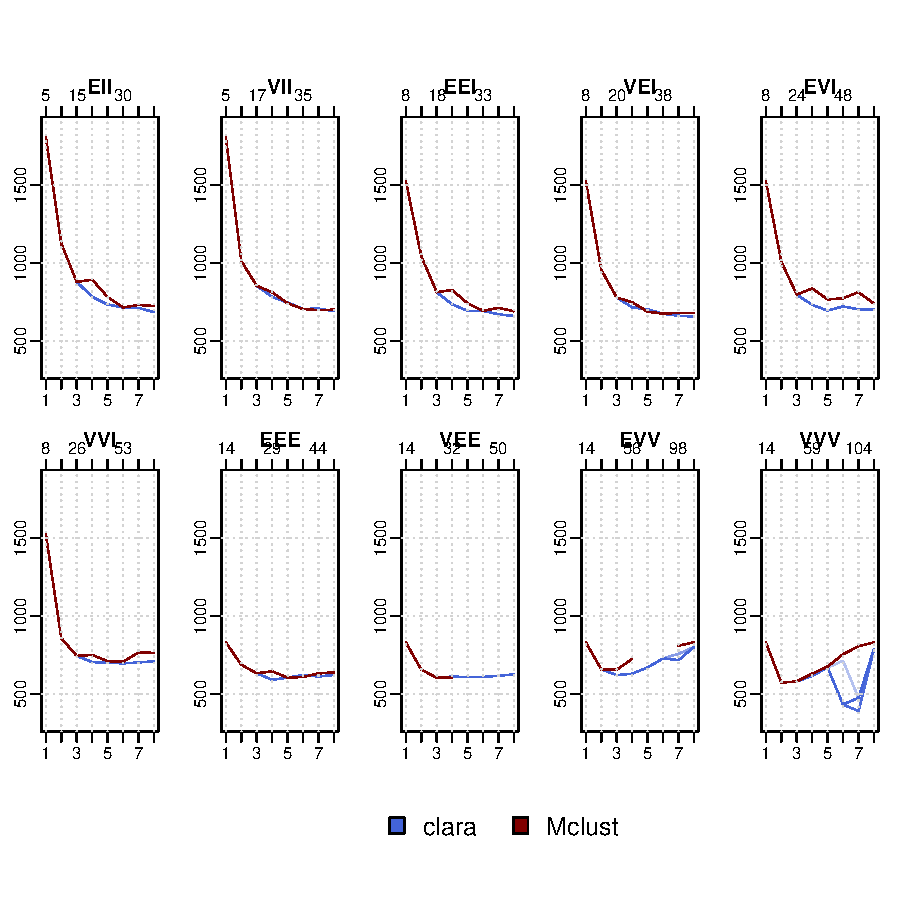
\includegraphics{chapter3-figtriris}
    \caption{The BIC values for the {\tt iris} data}
    \label{fig:triris}
    \end{Rgraph}
\end{figure}

The iris data originates from three types of plant species, which is not 
correctly identified by either {\tt norMmix} or {\tt mclust}. The best models
chosen are:

\begin{Schunk}
\begin{Soutput}
     model   count
[1,] "6 VVV" "18" 
[2,] "7 VVV" "7"  
\end{Soutput}
\end{Schunk}

both far from three components. Furthermore {\tt mclust} does not return values
for some combinations of {\tt k} and {\tt model}. It is not clear what causes 
this, as a call to {\tt Mclust} simply returns {\tt NULL}.

Lastly, the data {\tt loss}, from the {\tt copula} package \cite{cop18}. This 
data is described as "Indemnity payment and allocated loss adjustment expense 
from an insurance company." It consists of $1500$ observations with $4$ 
variables. The BIC values are shown in \ref{fig:loss}

\begin{figure}[h!]
    \begin{Rgraph}[0.9]
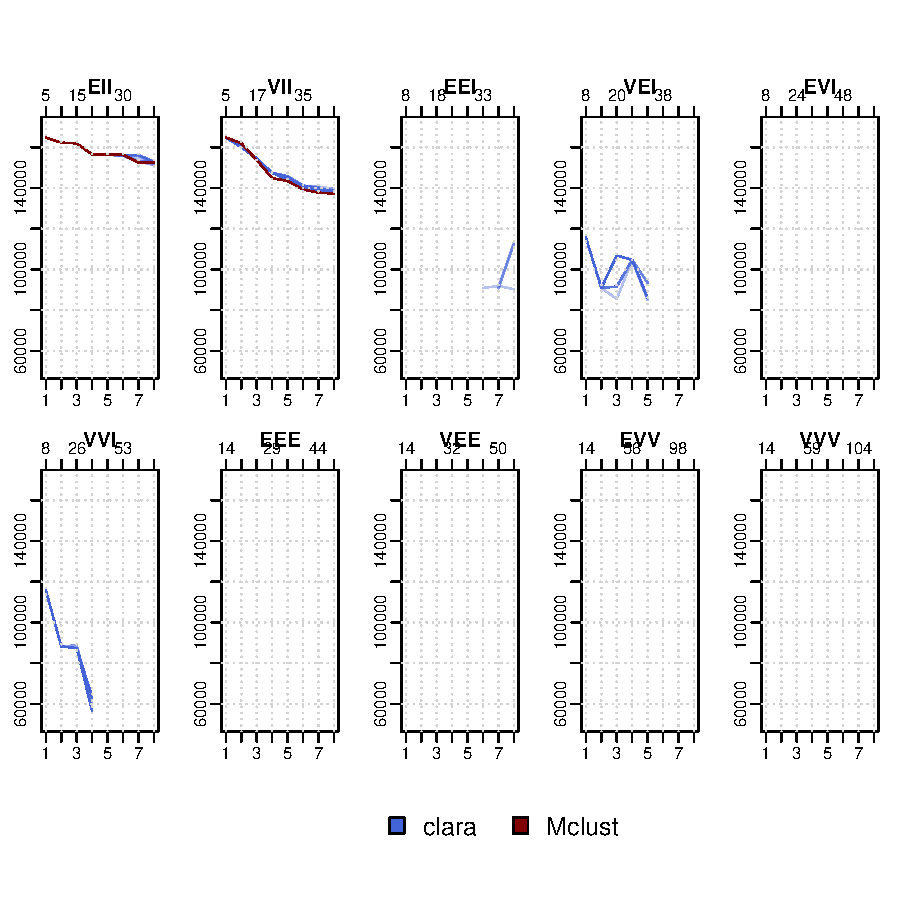
\includegraphics{chapter3-figloss}
    \caption{Loss data}
    \label{fig:loss}
    \end{Rgraph}
\end{figure}

The data resists any attempt at fitting. {\tt mclust} returns {\tt NULL}, as 
with {\tt iris}. In {\tt norMmix}, the {\tt optim} function encounters an error.

\begin{Schunk}
\begin{Sinput}
>     data(loss, package="copula")
>     to <- try(norMmixMLE(loss, k=3, model="EEI"))
\end{Sinput}
\begin{Soutput}
initial  value 58082.835867 
iter  10 value 56418.201189
iter  20 value 53014.372756
iter  30 value 49490.970255
iter  40 value 46802.853871
\end{Soutput}
\begin{Sinput}
>     print(to)
\end{Sinput}
\begin{Soutput}
[1] "Error in optim(initpar., neglogl, method = method, control = control) : \n  non-finite finite-difference value [6]\n"
attr(,"class")
[1] "try-error"
attr(,"condition")
<simpleError in optim(initpar., neglogl, method = method, control = control): non-finite finite-difference value [6]>
\end{Soutput}
\end{Schunk}


\chapter{Discussion}




one shortcoming is time inefficiency. largely due to implementation.
mclust has 16'000 lines of Fortran code, impossible in the scope of this thesis.

proof of concept??
definitely possible to do model selection using a general optimizer.

strong points:
'randomness' of clara/optim allows 'confidence intervalls' for selected model
flexibility of approach: given an logLik fctn can do mixture fitting w/ arbitrary
models

further study might include: other presumed component distributions, 'high' dimensions

failures of implementation: no lower boundary for variance, can lead to minuscule components
not as bad as it used to be.

%% and more
% \include{....}
 
%%%%%%%%%%%%%%%%%%%%%%%%%%%%%%%%%%%%%%%%%%%%%%%%%
%%% Bibliography                              %%%
%%%%%%%%%%%%%%%%%%%%%%%%%%%%%%%%%%%%%%%%%%%%%%%%%
\addtocontents{toc}{\vspace{.5\baselineskip}}
% \cleardoublepage
\phantomsection
\addcontentsline{toc}{chapter}{\protect\numberline{}{Bibliography}}
\bibliography{References}
%% All books from our library (SfS) are already in a BiBTeX file
%% 'Assbib.bib' (included here as well), using
% \bibliography{myReferences,Assbib}
% ---------------------------------- instead of the above

%%%%%%%%%%%%%%%%%%%%%%%%%%%%%%%%%%%%%%%%%%%%%%%%% 
%%% Appendices (if needed, e.g. for R code)   %%%
%%%%%%%%%%%%%%%%%%%%%%%%%%%%%%%%%%%%%%%%%%%%%%%%%
\addtocontents{toc}{\vspace{.5\baselineskip}}
\appendix
\chapter{\Rp Code}
\section{{\tt llnorMmix}}

\begin{Schunk}
\begin{Soutput}
#### the llnorMmix function, calculating log likelihood for a given
#### parameter vector
## Author: Nicolas Trutmann 2019-07-06
## Log-likelihood of parameter vector given data
#
# par:   parameter vector
# tx:    transposed sample matrix
# k:     number of components
# model: assumed distribution model of normal mixture
# trafo: either centered log ratio or logit
llnorMmix <- function(par, tx, k,
                      trafo=c("clr1", "logit"),
                      model=c("EII","VII","EEI","VEI","EVI",
                              "VVI","EEE","VEE","EVV","VVV")
                      )
{
    stopifnot(is.matrix(tx),
              length(k <- as.integer(k)) == 1, k >= 1)
    p <- nrow(tx)
#    x <- t(x) ## then only needed in   (x-mu[,i])^2  i=1..k
    # 2. transform
    model <- match.arg(model)
    trafo <- match.arg(trafo)
    l2pi <- log(2*pi)
    # 3. calc log-lik
    # get w
    w <- if (k==1) 1
         else switch(trafo,
                     "clr1" = clr1inv (par[1:(k-1)]),
                     "logit"= logitinv(par[1:(k-1)]),
                     stop("invalid 'trafo': ", trafo)
         )
    # start of relevant parameters:
    f <- k + p*k # weights -1 + means +1 => start of alpha
    # get mu
    mu <- matrix(par[k:(f-1L)], p,k)
    f1 <- f      # end of alpha if uniform
    f2 <- f+k-1L # end of alpha if var
    f1.1 <- f1 +1L # start of D. if alpha unif.
    f2.1 <- f1 + k # start of D. if alpha variable
    f11 <- f1 + p-1    # end of D. if D. uniform and alpha uniform
    f12 <- f1 +(p-1)*k # end    D. if D.   var   and alpha unif.
    f21 <- f2 + p-1    # end of D. if D. uniform and alpha variable
    f22 <- f2 +(p-1)*k # end of D. if D.   var   and alpha var.
    f11.1 <- f11 +1L # start of L if alpha unif  D unif
    f21.1 <- f21 +1L # start of L if alpha var   D unif
    f12.1 <- f12 +1L # start of L if alpha unif  D var
    f22.1 <- f22 +1L # start of L if alpha var   D var
    f111 <- f11 +   p*(p-1)/2 # end of L if alpha unif  D unif
    f211 <- f21 +   p*(p-1)/2 # end of L if alpha var   D unif
    f121 <- f12 + k*p*(p-1)/2 # end of L if alpha unif  D var
    f221 <- f22 + k*p*(p-1)/2 # end of L if alpha var   D var
    # initialize f(tx_i) i=1..n  vector of density values
    invl <- 0
    # calculate log-lik, see first case for explanation
    switch(model,
    "EII" = {
        alpha <- par[f]
        invalpha <- exp(-alpha)# = 1/exp(alpha)
        for (i in 1:k) {
            rss <- colSums(invalpha*(tx-mu[,i])^2)
            # this is vector of length n=sample size
            # calculates (tx-mu)t * Sigma^-1 * (tx-mu) for diagonal
            # cases.
            invl <- invl+w[i]*exp(-0.5*(p*(alpha+l2pi)+rss))
            # adds likelihood of one component to invl
            # the formula in exp() is the log of likelihood
            # still of length n
        }
    },
    # hereafter differences are difference in dimension in alpha and D.
    # alpha / alpha[i] and D. / D.[,i]
    "VII" = {
        alpha <- par[f:f2]
        for (i in 1:k) {
            rss <- colSums((tx-mu[,i])^2/exp(alpha[i]))
            invl <- invl+w[i]*exp(-0.5*(p*(alpha[i]+l2pi)+rss))
        }
    },
    "EEI" = {
        alpha <- par[f]
        D. <- par[f1.1:f11]
        D. <- c(-sum(D.),D.)
        D. <- D.-sum(D.)/p
        invD <- exp(alpha+D.)
        for (i in 1:k) {
            rss <- colSums((tx-mu[,i])^2/invD)
            invl <- invl+w[i]*exp(-0.5*(p*(alpha+l2pi)+rss))
        }
    },
    "VEI" = {
        alpha <- par[f:f2]
        D. <- par[f2.1:f21]
        D. <- c(-sum(D.), D.)
        D. <- D.-sum(D.)/p
        for (i in 1:k) {
            rss <- colSums((tx-mu[,i])^2/exp(alpha[i]+D.))
            invl <- invl+w[i]*exp(-0.5*(p*(alpha[i]+l2pi)+rss))
        }
    },
    "EVI" = {
        alpha <- par[f]
        D. <- matrix(par[f1.1:f12],p-1,k)
        D. <- apply(D.,2, function(j) c(-sum(j), j))
        D. <- apply(D.,2, function(j) j-sum(j)/p)
        for (i in 1:k) {
            rss <- colSums((tx-mu[,i])^2/exp(alpha+D.[,i]))
            invl <- invl+w[i]*exp(-0.5*(p*(alpha+l2pi)+rss))
        }
    },
    "VVI" = {
        alpha <- par[f:f2]
        D. <- matrix(par[f2.1:f22],p-1,k)
        D. <- apply(D.,2, function(j) c(-sum(j), j))
        D. <- apply(D.,2, function(j) j-sum(j)/p)
        for (i in 1:k) {
            rss <- colSums((tx-mu[,i])^2/exp(alpha[i]+D.[,i]))
            invl <- invl+w[i]*exp(-0.5*(p*(alpha[i]+l2pi)+rss))
        }
    },
    # here start the non-diagonal cases. main difference is the use
    # of backsolve() to calculate tx^t Sigma^-1 tx, works as follows:
    # assume Sigma = L D L^t, then Sigma^-1 = (L^t)^-1 D^-1 L^-1
    # y = L^-1 tx  => tx^t Sigma^-1 tx = y^t D^-1 y
    # y = backsolve(L., tx)
    "EEE" = {
        alpha <- par[f]
        D. <- par[f1.1:f11]
        D. <- c(-sum(D.), D.)
        D. <- D.-sum(D./p)
        invD <- exp(alpha+D.)
        L. <- diag(1,p)
        L.[lower.tri(L., diag=FALSE)] <- par[f11.1:f111]
        for (i in 1:k) {
            rss <- colSums(backsolve(L.,(tx-mu[,i]), upper.tri=FALSE)^2/invD)
            invl <- invl+w[i]*exp(-0.5*(p*(alpha+l2pi)+rss))
        }
    },
    "VEE" = {
        alpha <- par[f:f2]
        D. <- par[f2.1:f21]
        D. <- c(-sum(D.), D.)
        D. <- D.-sum(D./p)
        L. <- diag(1,p)
        L.[lower.tri(L., diag=FALSE)] <- par[f21.1:f211]
        for (i in 1:k) {
            rss <- colSums(backsolve(L., (tx-mu[,i]), upper.tri=FALSE)^2/exp(alpha[i]+D.))
            invl <- invl+w[i]*exp(-0.5*(p*(alpha[i]+l2pi)+rss))
        }
    },
    "EVV" = {
        alpha <- par[f]
        D. <- matrix(par[f1.1:f12],p-1,k)
        D. <- apply(D.,2, function(j) c(-sum(j), j))
        D. <- apply(D.,2, function(j) j-sum(j)/p)
        L.temp <- matrix(par[f12.1:f121],p*(p-1)/2,k)
        for (i in 1:k) {
            L. <- diag(1,p)
            L.[lower.tri(L., diag=FALSE)] <- L.temp[,i]
            rss <- colSums(backsolve(L., (tx-mu[,i]), upper.tri=FALSE)^2/exp(alpha+D.[,i]))
            invl <- invl+w[i]*exp(-0.5*(p*(alpha+l2pi)+rss))
        }
    },
    "VVV" = {
        alpha <- par[f:f2]
        D. <- matrix(par[f2.1:f22],p-1,k)
        D. <- apply(D.,2, function(j) c(-sum(j), j))
        D. <- apply(D.,2, function(j) j-sum(j)/p)
        invalpha <- exp(rep(alpha, each=p)+D.)
        L.temp <- matrix(par[f22.1:f221],p*(p-1)/2,k)
        L. <- diag(1,p)
        for (i in 1:k) {
            L.[lower.tri(L., diag=FALSE)] <- L.temp[,i]
            rss <- colSums(backsolve(L., (tx-mu[,i]), upper.tri=FALSE)^2/invalpha[,i])
            invl <- invl+w[i]*exp(-0.5*(p*(alpha[i]+l2pi)+rss))
        }
    },
    ## otherwise
    stop("invalid model:", model)
    )
    ## return  sum_{i=1}^n log( f(tx_i) ) :
    sum(log(invl))
}
sllnorMmix <- function(x, obj, trafo=c("clr1", "logit")) {
    stopifnot(is.character(model <- obj$model))
    trafo <- match.arg(trafo)
    llnorMmix(nMm2par(obj, model=model),
              tx = t(x), k = obj$k, model=model, trafo=trafo)
}
## log-likelihood function relying on mvtnorm function
#
# par:   parameter vector as calculated by nMm2par
# x:     matrix of samples
# k:     number of cluster
# trafo: transformation of weights
# model: assumed model of the distribution
llmvtnorm <- function(par, x, k,
                      trafo=c("clr1", "logit"),
                      model=c("EII","VII","EEI","VEI","EVI",
                              "VVI","EEE","VEE","EVV","VVV")
              )
{
    stopifnot(is.matrix(x),
              length(k <- as.integer(k)) == 1, k >= 1)
    model <- match.arg(model)
    trafo <- match.arg(trafo)
    p <- ncol(x)
    nmm <- par2nMm(par, p, k, model=model, trafo=trafo)
    ## FIXME (speed!):  dmvnorm(*, sigma= S) will do a chol(S) for each component
    ## -----  *instead* we already have LDL' and  chol(S) = sqrt(D) L' !!
    ## another par2*() function should give L and D, or from that chol(Sagma), rather than Sigma !
    w <- nmm$w
    mu <- nmm$mu
    sig <- nmm$Sigma
    y <- 0
    for (i in 1:k) {
        y <- y + w[i]*mvtnorm::dmvnorm(x,mean=mu[,i],sigma=sig[,,i])
    }
    sum(log(y))
}
\end{Soutput}
\end{Schunk}

\section{Example Simulation Script}

% TODO:
here e.g. 2init.R and write some remarks on it.

% outcommented \chapter{Complementary information}
\label{app:complement}

Additional material. For example long mathematical derivations could be
given in the appendix. Or you could include part of your code that is
needed in printed form. You can add several Appendices to your thesis (as
you can include several chapters in the main part of your work).

\section{Including \Rp code with verbatim}
A simple (rather too simple, see~\ref{App:listings}) way to include code or
{\it R} output is to use 
\texttt{verbatim}. It just prints the text however it is (including all
spaces, ``strange'' symbols,...) in a slightly different font.
\begin{verbatim}
## loading packages
library(RBGL)
library(Rgraphviz)
library(boot)

## global variables
X_MAX <- 150

   This allows me to put as many s  p a   c es   as I want.
I can also use \ and ` and & and all the rest that is usually only 
accepted in the math mode.

I can also make as 
                  many 
             line 
    breaks as 
I want... and
             where I want. 
\end{verbatim}

But really recommended,  much better is the following:

\section{Including \Rp code with the \emph{listings} package}\label{App:listings}
However, it is much nicer to use the \emph{listings} package to include \Rp
code in your report. It allows you to number the lines, color the comments
differently than the code, and so on.
All the following is produced by simply writing

or \verb!\lstinputlisting{/u/maechler/R/Pkgs/sfsmisc/R/ellipse.R}! :

\lstinputlisting{ellipse.R}% was /u/maechler/R/Pkgs/sfsmisc/R/ellipse.R

\section{Using Sweave to include \Rp code (and more) in your report}
The easiest (and most elegant) way to include \Rp code and its output (and
have all your figures up to date with your report) is to use Sweave. You
can find an introduction Sweave in \texttt{/u/sfs/StatSoftDoc/Sweave/Sweave-tutorial.pdf}.

%%% Local Variables: 
%%% mode: latex
%%% TeX-master: "BachelorThesisSfS"
%%% End: 

% outcommented \chapter{2nd Appendix: More sophisticated R code listing} \label{appendix-more-R}

Chapter-wise listing of parts of R code, using
\begin{itemize}
\item \texttt{firstline=n1}
\item \texttt{lastline=n2}
\item \texttt{title=<text>}
\end{itemize}
e.g., for the first example below
\begin{verbatim}
\lstinputlisting[firstline=1,lastline=32,
                 title= \texttt{read\_irwls\_fn.R}]{../RCode/read_irwls_fn.R}
\end{verbatim}

% \section{Chapter 2} \label{app 2}

% \lstinputlisting[firstline=1,lastline=77,
% title=\texttt{analytic\_efficiency.R}]{../RCode/analytic_efficiency.R}
% %\lstinputlisting[firstline=,lastline=]{../RCode/???.R}

\bigskip% or even  \clearpage

%-----------------------------------------------------------------------------------------
\section{Chapter 5} \label{app 5}

% \lstinputlisting[firstline=1,lastline=71,
%                  title=\texttt{loss-fn\_rotated.R}]{../RCode/loss-fn_rotated.R}
%\lstinputlisting[firstline=1,lastline=32,
%                 title= \texttt{read\_irwls\_fn.R}]{../RCode/read_irwls_fn.R}

\medskip
                 
%\lstinputlisting[firstline=1,lastline=45,title=\texttt{plot.psi.R}]{../RCode/plot.psi.R}
%\lstinputlisting[firstline=,lastline=]{../RCode/???.R}
%\lstinputlisting[firstline=,lastline=]{../RCode/???.R}

% \clearpage
%-----------------------------------------------------------------------------------------
% \section{Chapter 7} \label{app 7}

% \lstinputlisting[firstline=1,lastline=35,
%                  title= \texttt{stat.test} from \texttt{lmrob2-fn.R}]{../RCode/lmrob2-fn.R}
% \lstinputlisting[firstline=41,lastline=194,
%                  title=\texttt{M.optimal.ms} from \texttt{lmrob2-fn.R}]{../RCode/lmrob2-fn.R}
%\lstinputlisting[firstline=,lastline=]{../RCode/???.R}
%-----------------------------------------------------------------------------------------

%%% Local Variables:
%%% mode: latex
%%% TeX-master: "MasterThesisSfS"
%%% End:


%%%%%%%%%%%%%%%%%%%%%%%%%%%%%%%%%%%%%%%%%%%%%%%%%% 
%%% Declaration of originality (Do not remove!)%%%
%%%%%%%%%%%%%%%%%%%%%%%%%%%%%%%%%%%%%%%%%%%%%%%%%%
%% Instructions:
%% -------------
%% fill in the empty document confirmation-originality.pdf electronically
%% print it out and sign it
%% scan it in again and save the scan in this directory with name
%% confirmation-originality-scan.pdf 
%%
%% General info on plagiarism:
%% https://www.ethz.ch/students/en/studies/performance-assessments/plagiarism.html 
\cleardoublepage
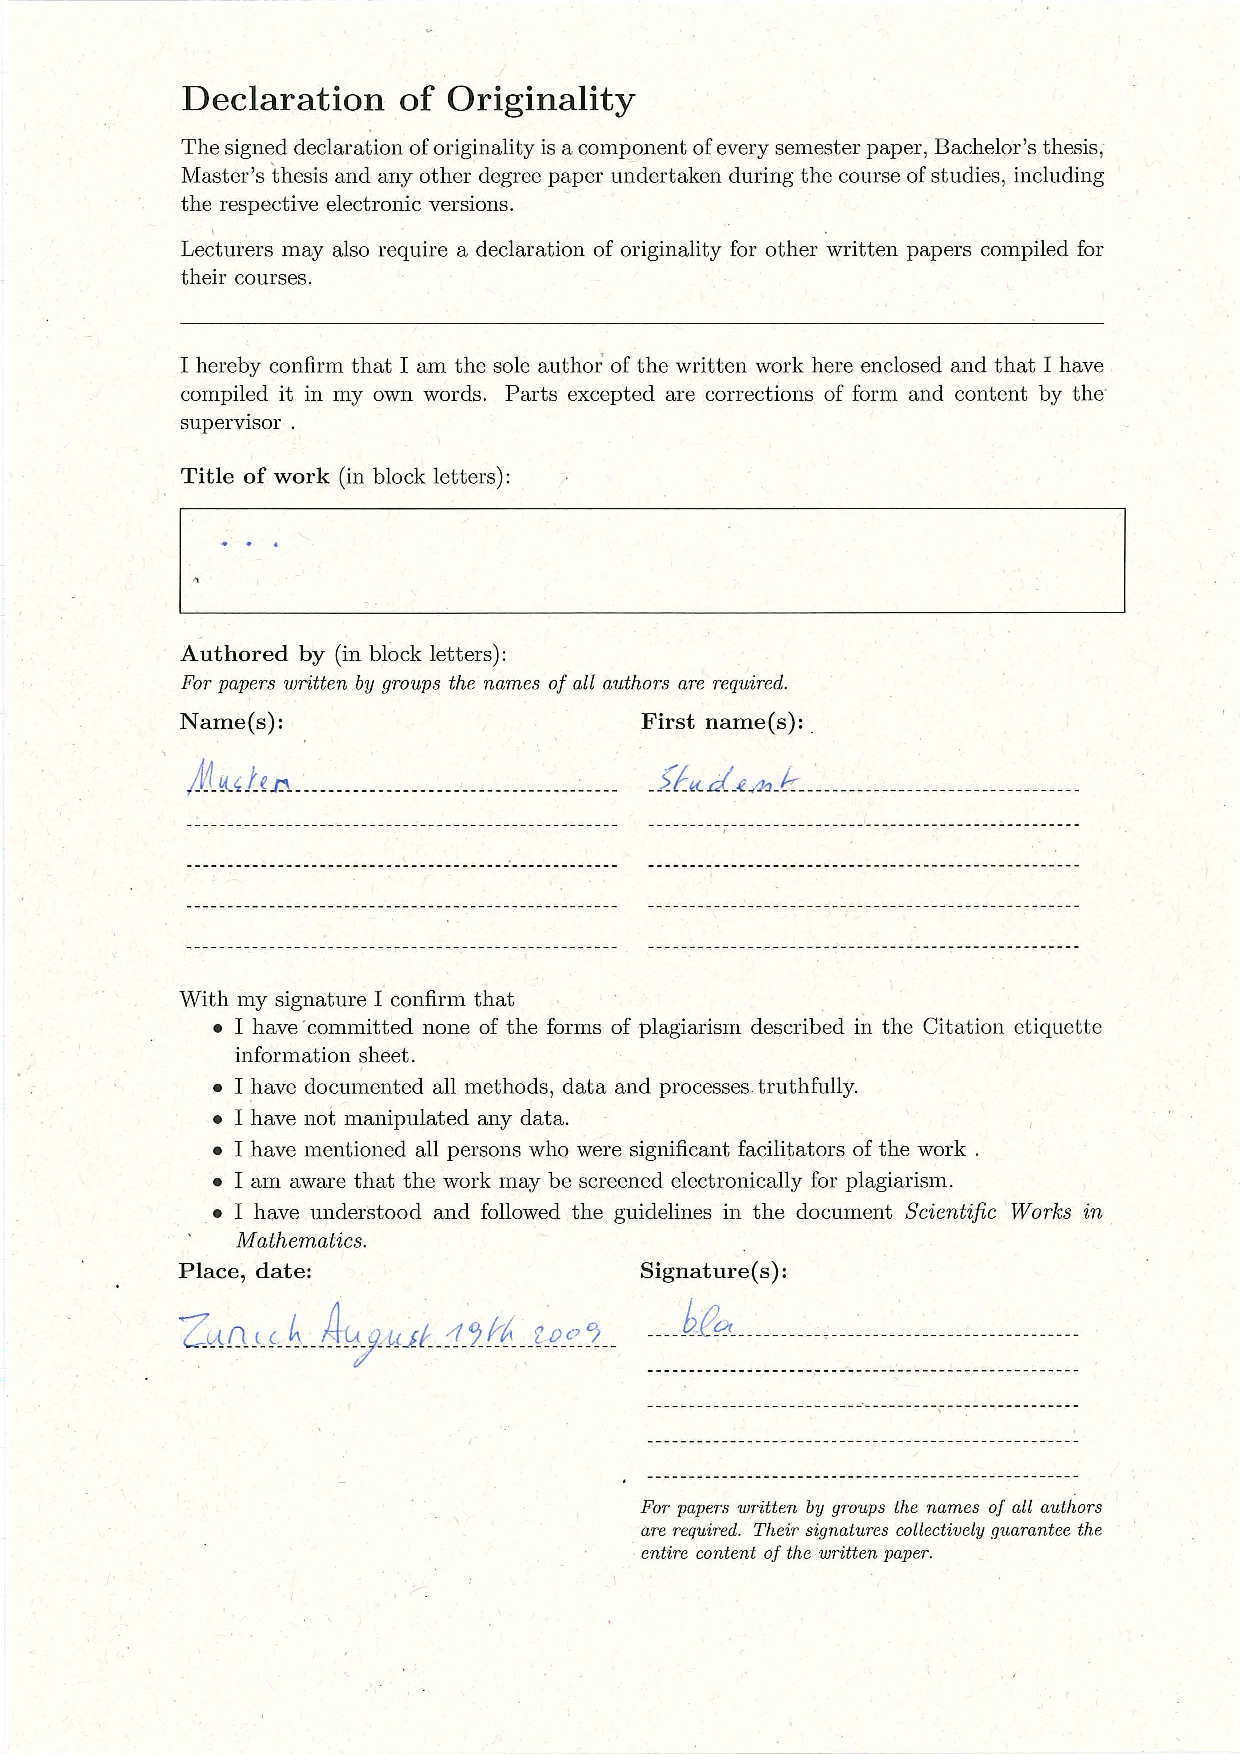
\includepdf[pages={-}, frame=true,scale=1]{confirmation-originality-scan.pdf}
\end{document}
